\documentclass[12pt,a4paper]{article}
\usepackage[utf8]{inputenc}
\usepackage[T1]{fontenc}
\usepackage[italian]{babel}
\usepackage{geometry}
\geometry{left=2.5cm, right=2.5cm, top=3.5cm, bottom=3.5cm}
\usepackage{amsmath,amssymb}
\usepackage{booktabs}
\usepackage{longtable}
\usepackage{array}
\usepackage{tabularx}
\usepackage{enumitem}
\usepackage{hyperref}
\usepackage{titlesec}
\usepackage{fancyhdr}
\usepackage{xcolor}
\usepackage{graphicx}
\usepackage{pgf-umlsd}
\usepackage{float}
\usepackage{tikz}
\usetikzlibrary{shapes.geometric, arrows.meta, positioning, fit, backgrounds}
\hypersetup{
    colorlinks=true,
    linkcolor=black,
    urlcolor=blue!60!black,
    citecolor=blue!60!black,
}
\pagestyle{fancy}
\fancyhf{}
\fancyhead[L]{\small Project Work APS -- Gruppo 20}
\fancyhead[R]{\small A.A.\ 2025/2026}
\fancyfoot[C]{\thepage}
\setlength{\headheight}{14pt}
\titleformat{\section}{\Large\bfseries}{}{0em}{}
\titleformat{\subsection}{\large\bfseries}{}{0em}{}
\titleformat{\subsubsection}{\normalsize\bfseries}{}{0em}{}
\newcommand{\pk}{\mathit{pk}}
\newcommand{\sk}{\mathit{sk}}

\begin{document}

% ══════════════════════════════════════════
% FRONTESPIZIO
% ══════════════════════════════════════════
\begin{titlepage}
\thispagestyle{empty}
\centering

\vspace*{1cm}

{\LARGE\scshape Università degli Studi di Salerno}\\[0.4cm]
{\large Dipartimento di Ingegneria dell'Informazione\\[0.2cm]
ed Elettrica e Matematica Applicata}\\[0.4cm]
{\large Corso di Laurea in Ingegneria Informatica}\\[1cm]


\includegraphics[width=50mm]{logo_unisa.png}\\[1.5cm]

\rule{\linewidth}{0.4pt}\\[0.4cm]
{\fontsize{22}{26}\selectfont\bfseries Algoritmi e Protocolli per la Sicurezza}\\[0.3cm]
\rule{\linewidth}{0.4pt}\\[1cm]

{\Large Project Work -- Gruppo 20}\\[2.5cm]

\begin{tabular}{lll}
\toprule
\textbf{\large Nome} & \textbf{\large Cognome} & \textbf{\large Matricola} \\
\midrule
{\large Chiara}   & {\large Amoroso}  & {\large IE22700309} \\[0.2cm]
{\large Antonio}  & {\large Esposito} & {\large IE22700003} \\
\bottomrule
\end{tabular}

\vfill

{\Large Anno Accademico 2025/2026}

\end{titlepage}


\begingroup
\setlength{\parskip}{0pt}
\linespread{0.94}\selectfont
\tableofcontents
\endgroup
\newpage
% ══════════════════════════════════════════════════════════════
% WP1: MODELLO DEL SISTEMA
% ══════════════════════════════════════════════════════════════

\section[WP1: Modello del Sistema]{WP\,1: Modello del Sistema}

\subsection{Funzionalit\`a del Sistema e Scenario Applicativo}

Il sistema ha l'obiettivo di digitalizzare in modo sicuro l'elezione per il rinnovo del Consiglio Direttivo Provinciale dell'Ordine degli Ingegneri. Il protocollo adotta un modello elettorale a \textbf{lista chiusa}, nel quale ciascun avente diritto pu\`o esprimere una sola preferenza verso una delle liste candidate ammesse.

La scelta della lista chiusa \`e motivata da esigenze di semplicit\`a, efficienza e verificabilit\`a. Rispetto a un'elezione con preferenza nominale, il dominio dei voti \`e ridotto a un insieme piccolo e predeterminato di codici, ad esempio $\{001, 002, 003\}$. Questo semplifica il formato della scheda elettronica, la validazione dei voti, la cifratura e lo scrutinio finale. Tale scelta consente inoltre di concentrare l'analisi sugli aspetti principali richiesti dal progetto: autenticazione degli elettori, pseudoanonimato, integrit\`a del registro, verificabilit\`a individuale e controllo pubblico del risultato.

Il sistema deve permettere agli ingegneri iscritti all'Albo e aventi diritto, di votare da remoto mediante un'interfaccia digitale. Al termine della votazione, la lista vincente viene determinata in base ai voti validamente registrati e i seggi sono assegnati secondo l'ordine di presentazione della lista.

Il ciclo di vita ideale dell'elezione si articola nelle seguenti fasi logiche.

\subsubsection*{Fase di configurazione}

L'autorit\`a competente pubblica l'elenco ufficiale delle liste ammesse e associa a ciascuna lista un codice identificativo univoco. Vengono inoltre definiti i parametri pubblici dell'elezione, il periodo di apertura e chiusura delle urne, gli attori coinvolti e le informazioni necessarie per consentire agli elettori di partecipare e agli osservatori di controllare il processo. L'elenco nominativo degli aventi diritto rimane nel dominio riservato della Registration Authority e non viene pubblicato sul Bulletin Board. Nella versione base del sistema vengono resi pubblici soltanto dati aggregati, come il numero totale degli aventi diritto.

\subsubsection*{Fase di autenticazione}

 L’elettore accede al sistema tramite credenziali istituzionali presso la Registration Authority. La RA verifica che l’utente sia iscritto all’Albo e abbia diritto a partecipare all’elezione. Se l’elettore non ha ancora ricevuto un’autorizzazione per la stessa elezione, la RA può procedere alla sua emissione. In caso di accessi successivi, l’autenticazione può essere ripetuta, ma la RA non rilascia una seconda autorizzazione. L’autenticazione è nominativa solo presso la RA e non deve essere trasferita al Bulletin Board o alla Tallying Authority. 

\subsubsection*{Fase di emissione e raccolta del voto}

Dopo l'autenticazione, l'elettore ottiene un'autorizzazione pseudonima che gli consente di depositare una scheda senza includere direttamente la propria identit\`a reale nel voto. L'elettore genera quindi una scheda elettronica protetta contenente il codice della lista scelta. La scheda viene inviata al Bulletin Board, che verifica la validit\`a dell'autorizzazione e registra il voto nel registro pubblico.

\subsubsection*{Fase di eventuale sostituzione del voto}

Prima della chiusura delle urne, il sistema pu\`o consentire all'elettore di sostituire la propria scheda con una nuova versione. Questa scelta mitiga alcuni scenari di coercizione o furto iniziale dell'autorizzazione, poich\'e una ricevuta ottenuta prima della chiusura non prova necessariamente quale voto sar\`a conteggiato alla fine. Ai fini dello scrutinio, per ciascun elettore pseudonimo viene considerata solo l'ultima versione valida registrata prima della chiusura.

\subsubsection*{Fase di scrutinio e verifica}

Alla chiusura delle urne, l'autorit\`a elettorale procede allo scrutinio dei soli voti validamente registrati. I voti non validi o malformati vengono separati e motivati. Sono quindi pubblicati il risultato finale, l'elenco delle schede finali conteggiate in forma pseudonima e le informazioni necessarie per controllare l'integrit\`a del registro, l'unicit\`a dei voti finali e la coerenza numerica dei totali.

La versione base del protocollo garantisce \textbf{verificabilit\`a individuale} e \textbf{controllo pubblico del registro}. La verificabilit\`a universale del tally \`e per\`o \textbf{parziale}: il pubblico non dispone, nella versione base, di una prova autonoma della corretta decifratura di ogni singola scheda. La correttezza dello scrutinio richiede quindi una fiducia residua nella Tallying Authority e nei commissari incaricati dello scrutinio.

% ──────────────────────────────────────────
\subsection{Identificazione degli Attori}

Al fine di garantire la separazione dei compiti e ridurre la fiducia in un'unica entit\`a centralizzata, il modello prevede sei attori logici, ciascuno con responsabilit\`a distinte.

\begin{small}
\begin{longtable}{>{\bfseries\raggedright}p{2.8cm} p{3.2cm} p{3.5cm} p{3.5cm}}
\toprule
Attore & Ruolo & Obiettivi principali & Risorse principali \\
\midrule
\endhead
Elettore &
Partecipante legittimo al voto. &
Autenticarsi, esprimere il proprio voto in segreto e verificare che la scheda sia stata inclusa nel registro. &
Credenziali istituzionali, dispositivo locale, autorizzazione pseudonima, informazioni necessarie alla verifica individuale. \\
\midrule
Registration Authority (RA) &
Sistema di autenticazione e validazione degli aventi diritto. &
Verificare l'identit\`a dell'elettore, controllare il diritto di voto e rilasciare al massimo una autorizzazione per elezione. &
Database riservato degli iscritti, credenziali istituzionali, chiave o meccanismo per emettere autorizzazioni. \\
\midrule
Tallying Authority (TA) &
Autorit\`a di scrutinio. &
Determinare l'insieme delle schede finali valide, eseguire lo scrutinio dopo la chiusura e pubblicare il risultato. &
Chiavi pubbliche dell'elezione, accesso controllato alla capacit\`a di decifrare durante lo scrutinio. \\
\midrule
Bulletin Board (BB) &
Registro pubblico append-only. &
Ricevere, verificare e pubblicare le schede registrate e gli eventi rilevanti dell'elezione. &
Registro pubblico consultabile, meccanismi di integrit\`a, ricevute di deposito. \\
\midrule
Commissari elettorali &
Soggetti incaricati di cooperare allo scrutinio. &
Autorizzare o partecipare allo scrutinio dopo la chiusura delle urne, riducendo il potere di una singola entit\`a. &
Credenziali operative o quote necessarie ad abilitare lo scrutinio, secondo il meccanismo definito nel WP2. \\
\midrule
Liste candidate / osservatori &
Osservatori del processo elettorale. &
Controllare in modo indipendente il registro pubblico, l'unicit\`a delle schede finali e la coerenza del risultato dichiarato. &
Accesso ai dati pubblici dell'elezione e agli strumenti di verifica. \\
\bottomrule
\end{longtable}
\end{small}
\begin{figure}[h!]
\centering
\resizebox{\textwidth}{!}{%
\begin{tikzpicture}[
    actor/.style={
        rectangle, rounded corners=6pt,
        draw=black, thick,
        minimum width=3.4cm, minimum height=1.1cm,
        text centered, font=\small\bfseries,
        align=center
    },
    arrow/.style={-{Stealth[length=6pt]}, thick},
    dasharrow/.style={-{Stealth[length=6pt]}, thick, dashed},
]

% Posizioni
\node[actor] (ra)          at (0, 8)     {Registration\\Authority (RA)};
\node[actor] (elettore)    at (0, 4)     {Elettore};
\node[actor] (bb)          at (6, 4)     {Bulletin\\Board (BB)};
\node[actor] (ta)          at (12, 4)    {Tallying\\Authority (TA)};
\node[actor] (commissari)  at (12, 0)    {Commissari\\Elettorali};
\node[actor] (osservatori) at (6, 0)     {Osservatori /\\Liste Candidate};

% RA -> Elettore (credenziali, andata)
\draw[arrow] ([xshift=-8pt]ra.south) -- 
    node[left, font=\scriptsize]{credenziali} 
    ([xshift=-8pt]elettore.north);

% Elettore -> RA (tau, ritorno)
\draw[arrow] ([xshift=8pt]elettore.north) -- 
    node[right, font=\scriptsize]{$\tau_i$} 
    ([xshift=8pt]ra.south);

% Elettore -> BB (pacchetto voto)
\draw[arrow] ([yshift=6pt]elettore.east) -- 
    node[above, font=\scriptsize]{pacchetto voto} 
    ([yshift=6pt]bb.west);

% BB -> Elettore (ricevuta ACK)
\draw[arrow] ([yshift=-6pt]bb.west) -- 
    node[below, font=\scriptsize]{ricevuta ACK} 
    ([yshift=-6pt]elettore.east);

% BB -> TA (schede cifrate)
\draw[dasharrow] (bb.east) -- 
    node[above, font=\scriptsize]{schede cifrate} 
    (ta.west);

% Commissari -> TA (quote)
\draw[arrow] (commissari.north) -- 
    node[right, font=\scriptsize]{quote $s_i$} 
    (ta.south);

% BB -> Osservatori (registro pubblico)
\draw[dasharrow] (bb.south) -- 
    node[right, font=\scriptsize]{registro pubblico} 
    (osservatori.north);

% TA -> Osservatori (risultato firmato) - passa sotto tutto
\draw[dasharrow] (ta.south) -- ++(0,-4.5) -- 
    node[below, font=\scriptsize]{risultato firmato}
    (osservatori.south);
    
% Box scrutinio
\begin{scope}[on background layer]
    \node[draw=black, thick, dashed, rounded corners=10pt,
          inner sep=16pt,
          fit=(ta)(commissari),
          label={[font=\scriptsize\itshape]above:Componente di Scrutinio}] {};
\end{scope}

\end{tikzpicture}%
}
\caption{Schema degli attori e flussi principali del protocollo.}
\label{fig:attori}
\end{figure}
% ──────────────────────────────────────────
\subsection{Modello di Minaccia e Avversari}

Si assume che gli avversari esterni siano computazionalmente limitati, cio\`e non siano in grado di rompere in tempo utile le primitive crittografiche adottate dal protocollo. Il modello considera sia avversari esterni, che possono osservare, ritrasmettere, modificare o iniettare messaggi, sia avversari interni, come RA, BB, TA o commissari elettorali curiosi o disonesti.

\subsubsection*{Attaccante passivo sulla rete}
\textbf{Tipologia:} passivo.\\
\textbf{Contesto e risorse:} un avversario osserva i messaggi scambiati durante la votazione, inclusi i pacchetti contenenti le schede cifrate inviate al Bulletin Board. Pu\`o raccogliere ciphertext, timestamp e metadati di rete, ma non possiede le chiavi private delle autorit\`a.\\
\textbf{Obiettivo:} dedurre la preferenza espressa da un elettore oppure correlare una scheda cifrata a un'identit\`a reale.\\


\subsubsection*{Attacchi alla segretezza del voto cifrato}
\textbf{Tipologia:} passivo o attivo, a seconda dello scenario.\\
\textbf{Contesto e risorse:} l'avversario pu\`o osservare solo ciphertext, conoscere alcune coppie voto-ciphertext ottenute a posteriori oppure generare voti scelti per studiare il comportamento della cifratura.\\
\textbf{Obiettivo:} sfruttare informazioni sui ciphertext per riconoscere voti uguali, costruire una tabella voto-ciphertext o dedurre la preferenza di altri elettori.\\


\subsubsection*{Elettore malizioso}
\textbf{Tipologia:} attivo.\\
\textbf{Contesto e risorse:} un elettore legittimo pu\`o tentare di votare pi\`u volte, inviare schede malformate, riutilizzare vecchi pacchetti, produrre sostituzioni non valide o contestare il proprio voto dopo averlo depositato.\\
\textbf{Obiettivo:} ottenere il conteggio di pi\`u voti, disturbare la votazione o generare ambiguit\`a nello scrutinio finale.\\


\subsubsection*{Contraffazione di autorizzazioni o pacchetti di voto}
\textbf{Tipologia:} attivo.\\
\textbf{Contesto e risorse:} un avversario tenta di costruire un pacchetto di voto apparentemente valido senza aver ricevuto una autorizzazione dalla RA, oppure tenta di modificare un pacchetto legittimo.\\
\textbf{Obiettivo:} introdurre voti fraudolenti nel Bulletin Board o alterare voti gi\`a registrati.\\


\subsubsection*{Replay attack}
\textbf{Tipologia:} attivo.\\
\textbf{Contesto e risorse:} un attaccante intercetta un pacchetto di voto valido gi\`a trasmesso da un elettore e lo ritrasmette invariato al BB.\\
\textbf{Obiettivo:} far conteggiare pi\`u volte lo stesso voto senza possedere nuove autorizzazioni valide.\\


\subsubsection*{Compromissione dello stato pseudonimo dell'elettore}
\textbf{Tipologia:} attivo.\\
\textbf{Contesto e risorse:} un avversario compromette il dispositivo dell'elettore o il suo archivio locale e ottiene parte dello stato pseudonimo associato all'elezione, come l'autorizzazione $\tau_i$, lo pseudonimo $p_i$, la chiave privata $sk_i^{vote}$, il segreto $t_i$, la versione corrente o le ricevute.\\
\textbf{Obiettivo:} impersonare l'elettore presso il BB, sostituire il voto prima della chiusura delle urne oppure impedire all'elettore di effettuare ulteriori sostituzioni.\\


\subsubsection*{RA curiosa o disonesta}
\textbf{Tipologia:} passivo / insider.\\
\textbf{Contesto e risorse:} la Registration Authority autentica nominativamente l'elettore e rilascia l'autorizzazione pseudonima. Nella versione base pu\`o conoscere il collegamento tra identit\`a reale e pseudonimo autorizzato.\\
\textbf{Obiettivo:} ricostruire l'associazione tra identit\`a reale e voto, soprattutto in caso di collusione con BB o TA.\\


\subsubsection*{TA o commissari disonesti}
\textbf{Tipologia:} attivo / insider.\\
\textbf{Contesto e risorse:} la Tallying Authority o alcuni commissari possono tentare di avviare lo scrutinio prima della chiusura, decifrare voti anticipatamente o alterare il conteggio.\\
\textbf{Obiettivo:} violare la segretezza del voto prima della chiusura o manipolare il risultato finale.\\


\subsubsection*{BB disonesto}
\textbf{Tipologia:} attivo / insider.\\
\textbf{Contesto e risorse:} il gestore del Bulletin Board pu\`o tentare di omettere una scheda, cancellare o modificare entry gi\`a pubblicate, riordinare il registro oppure mostrare viste diverse a elettori e osservatori.\\
\textbf{Obiettivo:} sopprimere voti legittimi, favorire una lista o rendere ambiguo lo stato finale dell'elezione.\\


\subsubsection*{Attacchi alle funzioni hash e alla hash chain}
\textbf{Tipologia:} attivo.\\
\textbf{Contesto e risorse:} un avversario tenta di trovare due entry diverse con lo stesso digest, oppure di sostituire una scheda gi\`a pubblicata con un'altra che mantenga invariati gli identificativi.\\
\textbf{Obiettivo:} alterare il registro pubblico senza che la modifica venga rilevata.\\


\subsubsection*{Dispositivo dell'elettore compromesso}
\textbf{Tipologia:} attivo.\\
\textbf{Contesto e risorse:} un malware sul dispositivo dell'elettore pu\`o leggere o modificare dati prima che vengano cifrati o firmati.\\
\textbf{Obiettivo:} alterare la preferenza prima della cifratura, impersonare l'elettore o indurlo a credere che sia stata registrata una scheda diversa.\\


\subsubsection*{Coercizione e vendita del voto}
\textbf{Tipologia:} attivo.\\
\textbf{Contesto e risorse:} un soggetto terzo pu\`o costringere o incentivare l'elettore a votare per una lista specifica e chiedere una prova del comportamento di voto.\\
\textbf{Obiettivo:} trasformare la ricevuta individuale in una prova del voto espresso.\\


\subsubsection*{Denial of Service}
\textbf{Tipologia:} attivo.\\
\textbf{Contesto e risorse:} un avversario genera molte richieste verso RA o BB durante il periodo di voto, anche senza possedere credenziali valide.\\
\textbf{Obiettivo:} impedire agli elettori legittimi di completare la procedura di voto.\\

\subsubsection*{Collusione tra autorit\`a}
\textbf{Tipologia:} insider / attivo o passivo.\\
\textbf{Contesto e risorse:} due o pi\`u entit\`a del sistema, ad esempio RA, BB, TA o un numero sufficiente di commissari, condividono le informazioni in loro possesso. La RA pu\`o conoscere l'associazione tra identit\`a reale e pseudonimo, il BB osserva le schede cifrate e gli pseudonimi pubblici, mentre la TA accede ai voti in chiaro durante lo scrutinio.\\
\textbf{Obiettivo:} ricostruire l'associazione tra identit\`a reale e preferenza di voto oppure anticipare o manipolare lo scrutinio.\\

% ──────────────────────────────────────────
\subsection{Propriet\`a di Sicurezza e Resilienza}

\subsubsection*{1.\ Confidenzialit\`a, segretezza e pseudoanonimato}

\begin{description}[style=nextline, leftmargin=1.2cm]
\item[\textbf{S.1} -- Segretezza del voto.] La preferenza espressa dal singolo elettore deve rimanere confidenziale durante la fase di raccolta e fino allo scrutinio. Un osservatore esterno, il Bulletin Board o la Registration Authority non devono poter ricavare la lista scelta a partire dalla scheda cifrata.
\item[\textbf{S.2} -- Pseudoanonimato.] Il sistema non garantisce anonimato forte, ma pseudoanonimato basato sulla separazione dei ruoli. La RA conosce l'identit\`a reale ma non il voto. Il BB vede lo pseudonimo $p_i$ e la scheda cifrata ma non l'identit\`a reale. La TA accede ai voti in chiaro solo durante lo scrutinio ma non riceve l'elenco nominativo.
\item[\textbf{S.3} -- Protezione dei canali.] Le comunicazioni tra elettore e RA, e tra elettore e BB, devono avvenire su canali protetti.
\item[\textbf{S.4} -- Cifratura probabilistica.] La cifratura del voto deve essere non deterministica, cio\`e deve usare casualit\`a fresca per ogni scheda.
\item[\textbf{S.5} -- Robustezza rispetto a ciphertext malformati.] Il sistema di raccolta non deve comportarsi come un oracolo capace di rivelare informazioni sul contenuto dei voti o sulla chiave privata di scrutinio.
\item[\textbf{S.6} -- Custodia distribuita della chiave di scrutinio.]
La chiave privata necessaria alla decifratura dei voti non deve essere utilizzabile autonomamente da una singola entit\`a prima della chiusura delle urne. Il sistema deve richiedere la cooperazione di almeno $t$ commissari su $n$ per recuperare la capacit\`a di scrutinio. Questa propriet\`a riduce il rischio di decifratura anticipata o unilaterale, pur non eliminando il rischio di collusione tra almeno $t$ commissari.
\end{description}

\subsubsection*{2.\ Integrit\`a, autenticit\`a e unicit\`a}

\begin{description}[style=nextline, leftmargin=1.2cm]
\item[\textbf{I.1} -- Integrit\`a delle schede registrate.] 
Le schede registrate nel Bulletin Board non devono poter essere alterate, cancellate, sostituite o riordinate senza che la modifica diventi rilevabile.

\item[\textbf{I.2} -- Registro append-only.] 
Ogni nuova entry viene aggiunta alla storia pubblica del registro; le entry gi\`a pubblicate non vengono modificate n\'e cancellate.

\item[\textbf{I.3} -- Integrit\`a tramite funzioni hash.] 
Il sistema deve usare funzioni hash crittografiche adeguate per proteggere gli identificativi delle schede e i collegamenti del registro.

\item[\textbf{A.1} -- Autenticit\`a degli elettori.] 
Solo gli ingegneri riconosciuti come aventi diritto e autenticati presso la Registration Authority possono partecipare alla votazione.

\item[\textbf{A.2} -- Unicit\`a del voto finale.] 
Ciascun avente diritto deve avere al pi\`u un voto valido finale. Eventuali sostituzioni devono essere riconducibili alla stessa autorizzazione pseudonima, senza rivelare l'identit\`a reale dell'elettore.

\item[\textbf{A.3} -- Non falsificabilit\`a.] 
Non deve essere possibile produrre autorizzazioni o pacchetti di voto apparentemente validi senza possedere le credenziali e i materiali crittografici necessari.

\item[\textbf{A.4} -- Resistenza al replay.] 
Un pacchetto gi\`a accettato non deve poter essere conteggiato pi\`u di una volta.

\item[\textbf{A.5} -- Tracciabilit\`a delle sostituzioni.] 
Se l'elettore sostituisce il voto, il registro deve conservare la storia delle versioni. Ai fini dello scrutinio viene considerata solo l'ultima versione valida registrata prima della chiusura delle urne.
\end{description}

\subsubsection*{3.\ Verificabilit\`a e trasparenza}

\begin{description}[style=nextline, leftmargin=1.2cm]
\item[\textbf{V.1} -- Verificabilit\`a individuale.] Ogni elettore deve poter verificare autonomamente che la propria scheda cifrata sia stata inclusa nel Bulletin Board.
\item[\textbf{V.2} -- Controllo pubblico del registro.] Osservatori esterni devono poter controllare l'integrit\`a del registro, la validit\`a delle firme e la presenza di una sola scheda finale per ciascuna autorizzazione pseudonima.
\item[\textbf{V.3} -- Verificabilit\`a universale parziale.] Chiunque deve poter verificare la coerenza numerica e la firma del risultato. Tuttavia, il pubblico non dispone di una prova crittografica della corretta decifratura di ogni singolo ciphertext.
\item[\textbf{T.1} -- Trasparenza degli algoritmi.] Il sistema deve utilizzare algoritmi e protocolli crittografici pubblicamente noti.
\item[\textbf{T.2} -- Esplicitazione delle assunzioni di fiducia.] Ogni assunzione di fiducia deve essere dichiarata e analizzata.
\item[\textbf{T.3} -- Verifica individuale e coercizione.] La ricevuta non contiene il voto in chiaro e la possibilit\`a di sostituire il voto prima della chiusura delle urne riduce il valore di una prova mostrata durante la votazione, ma non impedisce completamente la coercizione.
\end{description}

\subsubsection*{4.\ Efficienza e scalabilit\`a}

\begin{description}[style=nextline, leftmargin=1.2cm]
\item[\textbf{E.1} -- Efficienza lato elettore.] Le operazioni richieste al singolo elettore devono avere costi computazionali contenuti.
\item[\textbf{E.2} -- Efficienza lato Bulletin Board.] Per ogni voto accettato, il BB deve eseguire un numero limitato di operazioni, con costo per-voto sostanzialmente indipendente dal numero totale degli elettori.
\item[\textbf{E.3} -- Scalabilit\`a dello scrutinio.] Lo scrutinio deve crescere in modo ragionevole con il numero di schede finali (costo lineare).
\item[\textbf{E.4} -- Scalabilit\`a della verifica pubblica.] La verifica completa del registro ha costo lineare nel numero di entry pubblicate.
\end{description}

% ──────────────────────────────────────────
\subsection{Completezza}

Per completezza si intende il comportamento del sistema nel caso in cui tutte le parti coinvolte si comportino onestamente e seguano il protocollo. Sotto questa ipotesi:

\begin{itemize}
\item se l'ingegnere \`e iscritto all'Albo e si autentica correttamente presso la RA, riceve un'autorizzazione pseudonima valida e firmata;
\item il client dell'elettore conserva in modo persistente e protetto lo stato pseudonimo, comprendente $t_i$, $p_i$, $\tau_i$, $(\pk_i^{\mathit{vote}}, \sk_i^{\mathit{vote}})$, la versione corrente e le ricevute ottenute;
\item se l'elettore possiede un'autorizzazione valida e la corrispondente chiave pseudonima, pu\`o depositare una scheda cifrata presso il BB;
\item se il pacchetto \`e ben formato, firmato correttamente e inviato entro il periodo di apertura, il BB lo registra nella hash chain e restituisce una ricevuta firmata;
\item se l'elettore sostituisce il voto prima della chiusura, il BB registra la nuova versione senza cancellare le precedenti, fino a un massimo di $V_{\max}$ versioni per ciascun pseudonimo $p_i$;
\item alla chiusura delle urne, il BB pubblica un evento $\texttt{CLOSE}$ nella hash chain e firma lo stato finale producendo $\mathit{SIG}_{\mathit{close}}$, che identifica in modo univoco lo stato ufficiale del registro;
\item per ciascun pseudonimo $p_i$ viene selezionata l'ultima versione valida registrata prima di $\texttt{CLOSE}$;
\item con la cooperazione di almeno $t$ commissari, $K_{\mathit{wrap}}$ viene ricostruita tramite Shamir e $\sk_{\mathit{TA\_dec}}$ viene recuperata temporaneamente dall'apertura autenticata di $\mathit{blob}_{\mathit{TA}}$;
\item la TA decifra le schede finali valide, calcola i totali e pubblica il risultato firmato, riferito a $h_{\mathit{close}}$;
\item ogni elettore pu\`o verificare l'inclusione della propria scheda cifrata tramite la ricevuta e lo pseudonimo $p_i$;
\item chiunque pu\`o verificare l'integrit\`a del registro, la validit\`a delle firme $\tau_i$ e $\sigma_i$, ricalcolare i $\mathit{RID}_i$, controllare la corretta selezione delle schede finali e la coerenza numerica del risultato.
\end{itemize}

La completezza non implica anonimato perfetto, resistenza completa alla coercizione o verificabilit\`a crittografica completa dello scrutinio.

% ──────────────────────────────────────────
\subsection{Compromessi Progettuali e Assunzioni di Fiducia}

\subsubsection*{Verificabilit\`a individuale e resistenza alla coercizione}

Il sistema privilegia la verificabilit\`a individuale, ritenuta essenziale per la fiducia nel processo, ma dichiara che la resistenza alla coercizione non \`e pienamente garantita. La possibilit\`a di sostituire il voto prima della chiusura mitiga parzialmente il rischio, poich\'e una ricevuta ottenuta durante la votazione non prova necessariamente quale scheda sar\`a conteggiata alla fine. Il numero massimo di sostituzioni \`e limitato a $V_{\max}$ versioni per ciascun pseudonimo $p_i$, bilanciando la mitigazione della coercizione con la protezione contro la saturazione del registro.

\subsubsection*{Segretezza del voto e verificabilit\`a universale del tally}

Il sistema non pubblica la corrispondenza tra ogni scheda cifrata e il voto in chiaro. La verificabilit\`a universale del tally \`e solo parziale: il pubblico pu\`o verificare integrit\`a, firme $\tau_i$ e $\sigma_i$, versioni, unicit\`a per ciascun $p_i$ e coerenza numerica, ma non pu\`o verificare autonomamente la corretta decifratura di ogni singolo ciphertext. Una verificabilit\`a universale completa richiederebbe prove crittografiche di corretta decifratura, non incluse nel nucleo base.

\subsubsection*{Pseudoanonimato e separazione dei ruoli}

La RA autentica gli elettori e conosce il collegamento tra identit\`a reale e pseudonimo $p_i$. Il BB registra schede cifrate e pseudonimi ma non conosce l'identit\`a reale. La TA decifra durante lo scrutinio ma non riceve l'elenco nominativo. Se RA, BB e TA colludessero, oppure se venissero combinati log e metadati, lo pseudoanonimato potrebbe essere indebolito. Per questo motivo, il protocollo richiede una chiara separazione organizzativa e tecnica tra le entit\`a e una minimizzazione dei log non necessari.

\subsubsection*{Token non blindato}

Nella versione base, la RA vede lo pseudonimo $p_i$ e la chiave $\pk_i^{\mathit{vote}}$ prima di firmare l'autorizzazione $\tau_i$, e pu\`o quindi conservare il collegamento tra identit\`a reale e pseudonimo. L'adozione di blind signature richiederebbe un protocollo di firma cieca correttamente progettato e analizzato, con padding e controlli adeguati. Poiché tale costruzione non è inclusa nel nucleo base del progetto, si sceglie di non adottarla e di dichiarare esplicitamente il rischio residuo di collegabilità presso la RA.

\subsubsection*{Fiducia residua nella Tallying Authority}

Nella versione base, il pubblico non dispone di prove crittografiche complete per verificare ogni decifratura. Si assume che la TA e i commissari seguano la procedura. Il risultato \`e firmato dalla TA e vincolato allo stato finale $h_{\mathit{close}}$ del BB, garantendo che il tally si riferisca a uno stato del registro univoco e non ambiguo.

\subsubsection*{Integrit\`a e disponibilit\`a del Bulletin Board}

La hash chain rende rilevabili alterazioni, cancellazioni o riordinamenti successivi alla pubblicazione. Alla chiusura delle urne, il BB firma lo stato finale del registro tramite $\mathit{SIG}_{\mathit{close}} = \mathrm{Sign}(\sk_{\mathit{BB}}, (\mathit{election\_id}, h_{\mathit{close}}))$, impedendo la presentazione di viste divergenti del registro a soggetti diversi. Tuttavia, il protocollo non impedisce al BB di rifiutare o omettere una richiesta prima della sua prima pubblicazione. L'elettore deve conservare la ricevuta firmata e verificare l'inclusione della propria scheda.

\subsubsection*{Radice di fiducia iniziale}

L'autenticit\`a delle chiavi pubbliche dell'elezione si basa sulla pubblicazione sul portale istituzionale autenticato dell'Ordine degli Ingegneri. Tale canale costituisce la radice di fiducia iniziale del protocollo. Se il portale venisse compromesso, un attaccante potrebbe sostituire le chiavi pubbliche e intercettare o alterare la votazione. L'integrit\`a del portale \`e un'assunzione di fiducia infrastrutturale non risolvibile dal solo protocollo crittografico.

\subsubsection*{Persistenza dello stato dell'elettore}

Il protocollo assume che il dispositivo dell'elettore conservi in modo integro e protetto lo stato pseudonimo ($t_i$, $p_i$, $\sk_i^{\mathit{vote}}$, $\tau_i$, la versione corrente e le ricevute). In caso di perdita definitiva dello stato locale, l'elettore non pu\`o pi\`u depositare nuove schede n\'e sostituire il voto, ma l'ultima scheda validamente registrata nel BB resta conteggiata nello scrutinio.

\subsubsection*{Affidabilit\`a del dispositivo dell'elettore}

Il protocollo protegge i messaggi dopo la loro generazione, ma non pu\`o garantire che il dispositivo rispetti la volont\`a dell'elettore. Un malware potrebbe alterare il voto prima della cifratura, rubare $t_i$ o $\sk_i^{\mathit{vote}}$, o falsificare la verifica locale. Si assume che il dispositivo non sia compromesso.

\subsubsection*{Disponibilit\`a dell'infrastruttura}

Attacchi DoS, guasti di rete e indisponibilit\`a dei server devono essere mitigati tramite misure operative e infrastrutturali, come rate limiting, ridondanza e procedure di emergenza. Il protocollo crittografico non risolve queste minacce.

% ══════════════════════════════════════════════════════════════
% WP2: SOLUZIONE
% ══════════════════════════════════════════════════════════════

\section[WP2: Soluzione]{WP\,2: Soluzione}

\subsection{Strumenti crittografici utilizzati}

\begin{small}
\begin{longtable}{>{\raggedright}p{3.8cm} p{9.2cm}}
\toprule
\textbf{Strumento} & \textbf{Scopo nel protocollo} \\
\midrule
\endhead
Cifratura a chiave pubblica probabilistica &
Protegge il contenuto del voto. L'elettore cifra il codice della lista scelta con la chiave pubblica della TA. La cifratura usa casualit\`a fresca. Nel prototipo: RSA-OAEP. \\
\midrule
Firma digitale &
Garantisce autenticit\`a e integrit\`a dei principali messaggi. La RA firma le autorizzazioni, l'elettore firma i pacchetti di voto con la chiave pseudonima, il BB firma ricevute e stato finale del registro e la TA firma parametri pubblici e risultato finale. Nel prototipo: RSA-PSS con SHA-256. \\
\midrule
Funzione hash crittografica &
Calcolo di $p_i = H(t_i)$, identificativi delle schede ($\mathit{RID}_i$), costruzione della hash chain del BB. Nel prototipo: SHA-256. \\
\midrule
Autenticazione con password, salt e hash su TLS &
Autentica nominativamente l'elettore presso la RA. TLS protegge il canale; salt e hash evitano di memorizzare la password in chiaro. \\
\midrule
Registro append-only con hash chain &
Permette di rilevare alterazioni, cancellazioni, inserimenti o riordinamenti. Ogni entry viene collegata alla precedente tramite hash. \\
\midrule
Secret Sharing di Shamir &
Custodia distribuita del segreto di wrapping. Shamir viene applicato a $K_{\mathit{wrap}}$, dal quale vengono derivate $K_{\mathit{enc}}$ e $K_{\mathit{mac}}$. Almeno $t$ commissari su $n$ possono ricostruire $K_{\mathit{wrap}}$. \\
\midrule
Protezione simmetrica Encrypt-then-Authenticate &
Protegge la chiave $\sk_{\mathit{TA\_dec}}$ tramite chiavi indipendenti derivate da $K_{\mathit{wrap}}$ con HKDF-SHA256: AES-256-CBC con padding PKCS7 per la cifratura e HMAC-SHA256 per l'autenticazione del ciphertext e del contesto. \\
\bottomrule
\end{longtable}
\end{small}

Non vengono utilizzate costruzioni crittografiche manuali o non standard. Shamir Secret Sharing viene usato solo come meccanismo di custodia distribuita e non realizza una vera decifratura a soglia.

\subsection{Sintesi delle chiavi}

\begin{small}
\begin{longtable}{>{\raggedright}p{2.5cm} >{\raggedright}p{2.5cm} p{8cm}}
\toprule
\textbf{Chiave} & \textbf{Proprietario} & \textbf{Uso nel protocollo} \\
\midrule
\endhead
$\pk_{\mathit{TA\_enc}}$ / $\sk_{\mathit{TA\_dec}}$ & TA &
Cifratura e decifratura dei voti. $\sk_{\mathit{TA\_dec}}$ viene protetta tramite $K_{\mathit{enc}}$ e $K_{\mathit{mac}}$, derivate da $K_{\mathit{wrap}}$, e recuperata solo durante lo scrutinio. \\
\midrule
$\pk_{\mathit{TA\_sig}}$ / $\sk_{\mathit{TA\_sig}}$ & TA &
Firma dei parametri pubblici e del risultato finale. Coppia distinta dalla precedente. \\
\midrule
$\pk_{\mathit{RA}}$ / $\sk_{\mathit{RA}}$ & RA &
Firma delle autorizzazioni pseudonime. Il BB usa $\pk_{\mathit{RA}}$ per verificarle. \\
\midrule
$\pk_{\mathit{BB}}$ / $\sk_{\mathit{BB}}$ & BB &
Firma delle ricevute di deposito (ACK) e dello stato finale del registro
($\mathrm{SIG}_{\mathit{close}}$).\\
\midrule
$\pk_i^{\mathit{vote}}$ / $\sk_i^{\mathit{vote}}$ & Elettore &
Coppia pseudonima generata per la singola elezione. $\sk_i^{\mathit{vote}}$ firma il pacchetto di voto. \\
\midrule
$t_i$ & Elettore &
Segreto casuale generato localmente, dal quale l'elettore deriva lo pseudonimo $p_i$. Non viene mai trasmesso al BB. Serve all'elettore per ricalcolare $p_i$ e ritrovare la propria entry durante la verifica individuale. \\
\midrule
$p_i = H(t_i)$ & Elettore / pubblico &
Pseudonimo pubblico dell'elettore. La titolarit\`a del voto non \`e dimostrata dalla conoscenza di $t_i$, ma dal possesso della chiave privata $\sk_i^{\mathit{vote}}$, che consente di produrre la firma $\sigma_i$ sul pacchetto di voto. \\
\midrule
$K_{\mathit{wrap}}$ & Setup / Commissari &
Segreto casuale di 32 byte usato come materiale radice per derivare $K_{\mathit{enc}}$ e $K_{\mathit{mac}}$. Suddiviso tra i commissari tramite Shamir. \\
\midrule
$K_{\mathit{enc}}$ / $K_{\mathit{mac}}$ & Setup / TA &
Chiavi indipendenti derivate da $K_{\mathit{wrap}}$ con HKDF-SHA256: $K_{\mathit{enc}}$ per AES-256-CBC e $K_{\mathit{mac}}$ per HMAC-SHA256. \\
\midrule
$s_1, \ldots, s_n$ & Commissari &
Quote Shamir di $K_{\mathit{wrap}}$. Almeno $t$ quote sono necessarie per ricostruire $K_{\mathit{wrap}}$. \\
\midrule
$\mathit{blob}_{\mathit{TA}}$ & TA / sistema &
Contenitore formato da contesto, $\mathit{election\_id}$, IV, ciphertext e MAC. \\
\midrule
$\mathit{salt}_i$, $\mathit{verifier}_i$ & RA &
Autenticazione dell'elettore. La password non \`e memorizzata in chiaro. \\
\bottomrule
\end{longtable}
\end{small}

% ──────────────────────────────────────────
\subsection{Fase 0 --- Configurazione del sistema}

Prima dell'apertura delle urne, la commissione elettorale configura l'elezione. Vengono pubblicati: $\mathit{election\_id}$, elenco delle liste ammesse con codice identificativo, periodo di apertura e chiusura delle urne, numero totale degli aventi diritto, $\pk_{\mathit{TA\_enc}}$, $\pk_{\mathit{TA\_sig}}$, $\pk_{\mathit{RA}}$, $\pk_{\mathit{BB}}$, i parametri pubblici dello schema a soglia ($t$, $n$) e il numero massimo di versioni consentite per ciascun pseudonimo ($V_{\max}$, ad esempio $V_{\max} = 3$).

I parametri e le chiavi pubbliche dell'elezione vengono pubblicati prima dell'apertura sul portale istituzionale autenticato dell'Ordine degli Ingegneri. Tale canale costituisce la \textbf{radice di fiducia iniziale} del protocollo: ogni elettore e osservatore pu\`o verificare l'autenticit\`a delle chiavi pubbliche confrontandole con quelle pubblicate sul portale ufficiale.

La TA genera due coppie di chiavi distinte: una per la cifratura e decifratura dei voti $(\pk_{\mathit{TA\_enc}}, \sk_{\mathit{TA\_dec}})$ e una per firmare parametri e risultati $(\pk_{\mathit{TA\_sig}}, \sk_{\mathit{TA\_sig}})$.

\subsubsection*{Autenticazione dei parametri pubblici}

I parametri pubblici sono serializzati in modo canonico e deterministico. Il payload include contesto, versione, $\mathit{election\_id}$, liste, apertura, chiusura, numero aventi diritto, $V_{\max}$, soglia $(t,n)$ e chiavi pubbliche TA, RA e BB.
\[
\mathit{params\_hash} = \mathrm{SHA\mbox{-}256}(\mathrm{CanonicalSerialize}(\mathit{payload}))
\]
\[
\mathit{SIG}_{\mathit{params}} = \mathrm{Sign}(\sk_{\mathit{TA\_sig}},\; \mathrm{CanonicalSerialize}(\mathit{payload}))
\]
$\mathit{params\_hash}$ e $\mathit{SIG}_{\mathit{params}}$ non fanno parte del payload. Ciascun componente ricalcola l'hash e verifica la firma con $\pk_{\mathit{TA\_sig}}$. Nel prototipo viene usato RSA-PSS con SHA-256.

La RA mantiene internamente l'elenco nominativo degli aventi diritto, che non viene pubblicato.

Il BB inizializza il registro pubblico append-only con il primo valore della hash chain:
\[
h_0 = H(\texttt{"BB-GENESIS"} \| \mathit{election\_id} \| \mathit{params\_hash})
\]

\subsubsection*{Custodia distribuita della chiave di scrutinio tramite Shamir}

La chiave privata $\sk_{\mathit{TA\_dec}}$ non viene divisa direttamente. La TA genera $K_{\mathit{wrap}}$ come segreto casuale di 32 byte. Da $K_{\mathit{wrap}}$ vengono derivate con HKDF-SHA256 due chiavi indipendenti di 32 byte, $K_{\mathit{enc}}$ e $K_{\mathit{mac}}$:
\[
K_{\mathit{enc}}
=
\mathrm{HKDF\mbox{-}SHA256}
(K_{\mathit{wrap}},\mathit{info}_{\mathit{enc}})
\]
\[
K_{\mathit{mac}}
=
\mathrm{HKDF\mbox{-}SHA256}
(K_{\mathit{wrap}},\mathit{info}_{\mathit{mac}})
\]
La chiave privata TA serializzata viene sottoposta a padding PKCS7 e cifrata con AES-256-CBC usando un IV casuale:
\[
C = \mathrm{AES\mbox{-}256\mbox{-}CBC}_{K_{\mathit{enc}}}(\mathit{IV},\; \mathrm{PKCS7}(\mathrm{Serialize}(\sk_{\mathit{TA\_dec}})))
\]
Viene poi calcolato HMAC-SHA256 sulla serializzazione canonica di contesto, $\mathit{election\_id}$, IV e ciphertext:
\[
\mathit{MAC} = \mathrm{HMAC\mbox{-}SHA256}(K_{\mathit{mac}},\; \mathrm{CanonicalSerialize}(\mathit{context}, \mathit{election\_id}, \mathit{IV}, C))
\]
$\mathit{blob}_{\mathit{TA}}$ contiene contesto, $\mathit{election\_id}$, IV, ciphertext e MAC:
\[
\mathit{blob}_{\mathit{TA}} = (\mathit{context}, \mathit{election\_id}, \mathit{IV}, C, \mathit{MAC})
\]
La costruzione \`e Encrypt-then-Authenticate. Il MAC viene verificato prima della decifratura CBC e prima della rimozione del padding; un MAC non valido produce un errore crittografico generico.

$K_{\mathit{wrap}}$ viene suddivisa tra i commissari tramite Shamir Secret Sharing con parametri $(t, n)$ configurabili. Nel profilo dimostrativo WP4 sono usati $t = 3$ e $n = 5$. Shamir costruisce un polinomio casuale di grado $t-1$ in un campo finito $\mathbb{Z}_q$, dove $q$ \`e un primo maggiore di $K_{\mathit{wrap}}$:
\[
g(x) = K_{\mathit{wrap}} + a_1 x + a_2 x^2 + \cdots + a_{t-1} x^{t-1} \pmod{q}
\]

con coefficienti $a_1, \ldots, a_{t-1}$ scelti casualmente in $\mathbb{Z}_q$. Ogni commissario $i$ riceve la quota $s_i = (i,\, g(i) \bmod q)$. Almeno $t$ quote con indici distinti permettono di ricostruire $K_{\mathit{wrap}} = g(0)$ tramite interpolazione di Lagrange; con meno di $t$ quote non si ottiene alcuna informazione su $K_{\mathit{wrap}}$.

Una singola quota Shamir non \`e verificabile autonomamente in modo crittografico. Una quota alterata produce una $K_{\mathit{wrap}}$ errata, che viene rilevata al momento dell'apertura autenticata di $\mathit{blob}_{\mathit{TA}}$: la verifica HMAC fallisce, impedendo la decifratura CBC e il recupero di $\sk_{\mathit{TA\_dec}}$.

Dopo la distribuzione, $K_{\mathit{wrap}}$ in chiaro e $\sk_{\mathit{TA\_dec}}$ in chiaro vengono eliminate dall'ambiente di configurazione.

% ──────────────────────────────────────────
\subsection{Fase 1 --- Autenticazione ed emissione dell'autorizzazione pseudonima}

L'elettore accede al portale della RA usando le proprie credenziali istituzionali. Nel caso base, la RA memorizza per ciascun utente:
\[
\mathit{verifier}_i = \mathrm{PasswordHash}(\mathit{password}_i, \mathit{salt}_i)
\]

Se l'autenticazione ha successo, la RA verifica che l'utente sia nell'elenco degli aventi diritto e non abbia gi\`a ricevuto un'autorizzazione. L'elettore genera localmente:
\begin{itemize}
\item $t_i$: un segreto casuale valido solo per questa elezione, che non verr\`a mai trasmesso al BB;
\item $p_i = H(t_i)$: lo pseudonimo pubblico, derivato dal segreto tramite hash;
\item $(\pk_i^{\mathit{vote}}, \sk_i^{\mathit{vote}})$: una coppia di chiavi pseudonima per firmare il voto.
\end{itemize}

L'elettore invia alla RA lo pseudonimo pubblico e la chiave pseudonima:
\[
M_{\mathit{AUTH}} = (\mathit{election\_id}, p_i, \pk_i^{\mathit{vote}})
\]

La RA firma il messaggio e restituisce l'autorizzazione:
\[
\tau_i = \mathrm{Sign}(\sk_{\mathit{RA}}, M_{\mathit{AUTH}})
\]

Poich\'e $M_{\mathit{AUTH}}$ contiene solo $p_i$ e non $t_i$, la firma $\tau_i$ \`e verificabile da chiunque conosca $p_i$ e $\pk_{\mathit{RA}}$, senza rivelare il segreto $t_i$. La RA registra che l'elettore ha gi\`a ricevuto un'autorizzazione. Dopo l'emissione dell'autorizzazione, il client dell'elettore conserva in modo persistente e protetto lo stato pseudonimo relativo all'elezione, comprendente $t_i$, $p_i$, la coppia $(\pk_i^{\mathit{vote}}, \sk_i^{\mathit{vote}})$, l'autorizzazione $\tau_i$, la versione corrente $v_i$ e le ricevute ottenute dal Bulletin Board. La chiusura e la successiva riapertura dell'applicazione non comportano quindi la perdita di tali informazioni. Il metodo concreto di memorizzazione protetta sar\`a definito e implementato nel WP4. Nella versione base, la RA conosce il collegamento tra identit\`a reale, pseudonimo $p_i$ e chiave $\pk_i^{\mathit{vote}}$, ma non conosce la preferenza.

\begin{figure}[h!]
\centering
\resizebox{\textwidth}{!}{%
\begin{tikzpicture}[
    actor/.style={
        rectangle, rounded corners=6pt,
        draw=black, thick,
        minimum width=3.4cm, minimum height=1.1cm,
        text centered, font=\small\bfseries,
        align=center
    },
    arrow/.style={-{Stealth[length=6pt]}, thick},
    note/.style={font=\scriptsize, align=center},
]

% Attori
\node[actor] (elettore) at (0,0)  {Elettore};
\node[actor] (ra)       at (10,0) {Registration\\Authority (RA)};

% Linee vita
\draw[thick, dashed] (0,-0.55) -- (0,-14);
\draw[thick, dashed] (10,-0.55) -- (10,-14);

% Separatori fasi
\draw[gray, thin] (0,-4.0) -- (10,-4.0);
\draw[gray, thin] (0,-8.0) -- (10,-8.0);

% Etichette fasi centrate sopra i separatori
\node[font=\scriptsize\itshape] at (5,-3.7) 
    {--- Fase 2: Generazione locale dello pseudonimo ---};
\node[font=\scriptsize\itshape] at (5,-7.7) 
    {--- Fase 3: Emissione autorizzazione ---};
\node[font=\scriptsize\itshape] at (5,-1.0) 
    {--- Fase 1: Autenticazione ---};

%% FASE 1
\draw[arrow] (0,-2.0) -- 
    node[above, note]{(username, password)} 
    (10,-2.0);

\node[note, anchor=west] at (10.3,-2.5) {verifica password};
\node[note, anchor=west] at (10.3,-3.3) {controlla diritto di voto};

%% FASE 2
\node[note, anchor=east] at (-0.3,-4.8) 
    {genera $t_i$ casuale};
\node[note, anchor=east] at (-0.3,-5.6) 
    {calcola $p_i = H(t_i)$};
\node[note, anchor=east] at (-0.3,-6.4) 
    {genera coppia pseudonima};
\node[note, anchor=east] at (-0.3,-7.2) 
    {$(pk^{vote}_{i},\, sk^{vote}_{i})$};

%% FASE 3
\draw[arrow] (0,-8.5) -- 
    node[above, note]
    {$M_{AUTH} = (\mathit{election\_id},\; p_i,\; pk^{vote}_{i})$} 
    (10,-8.5);

\node[note, anchor=west] at (10.3,-9.8) 
    {$\tau_i = \mathrm{Sign}(sk_{RA},\, M_{AUTH})$};

\draw[arrow] (10,-11.0) -- 
    node[above, note]{$\tau_i$} 
    (0,-11.0);

\node[note, anchor=east] at (-0.3,-12.2) 
    {salva stato pseudonimo:};
\node[note, anchor=east] at (-0.3,-12.9) 
    {$(t_i,\, p_i,\, \tau_i,\, pk^{vote}_{i},\, sk^{vote}_{i},\, v_i{=}1)$};
\end{tikzpicture}%
}
\caption{Diagramma di sequenza: autenticazione ed emissione 
dell'autorizzazione pseudonima (Fase 1).}
\label{fig:autenticazione}
\end{figure}
% ──────────────────────────────────────────
\subsection{Fase 2 --- Preparazione e invio del voto}

L'elettore seleziona il codice della lista prescelta $j \in \{001, \ldots, K\}$ e lo cifra con casualit\`a fresca~$r$:
\[
c = \mathrm{Enc}(\pk_{\mathit{TA\_enc}}, j;\; r)
\]

Per il primo deposito, l'elettore imposta $v_i = 1$ e costruisce il messaggio:
\[
M_{\mathit{BALLOT}_i} = (\mathit{election\_id}, p_i, c, \pk_i^{\mathit{vote}}, v_i)
\]

Firma il messaggio con la chiave pseudonima:
\[
\sigma_i = \mathrm{Sign}(\sk_i^{\mathit{vote}}, M_{\mathit{BALLOT}_i})
\]

Il pacchetto inviato al Bulletin Board \`e:
\[
\mathit{MSG} = (c, p_i, \pk_i^{\mathit{vote}}, \tau_i, v_i, \sigma_i)
\]

Il pacchetto non contiene l'identit\`a reale dell'elettore n\'e il segreto $t_i$. Lo pseudonimo $p_i$ \`e un hash unidirezionale: chiunque pu\`o usarlo per verificare $\tau_i$ e $\sigma_i$ con le rispettive chiavi pubbliche, ma non pu\`o risalire a $t_i$. La firma pseudonima $\sigma_i$ dimostra il possesso della chiave $\sk_i^{\mathit{vote}}$: il solo possesso di $p_i$ e $\tau_i$ non \`e sufficiente per generare o sostituire un voto valido.

% ──────────────────────────────────────────
\subsection{Fase 3 --- Raccolta e validazione sul Bulletin Board}

Quando il BB riceve $\mathit{MSG} = (c, p_i, \pk_i^{\mathit{vote}}, \tau_i, v_i, \sigma_i)$, esegue i seguenti controlli:

\begin{enumerate}
\item Verifica l'autorizzazione della RA: $\mathrm{Verify}(\pk_{\mathit{RA}}, (\mathit{election\_id}, p_i, \pk_i^{\mathit{vote}}), \tau_i) = 1$.
\item Verifica la firma pseudonima: $\mathrm{Verify}(\pk_i^{\mathit{vote}}, (\mathit{election\_id}, p_i, c, \pk_i^{\mathit{vote}}, v_i), \sigma_i) = 1$.
\item Controlla che l'elezione sia ancora aperta.
\item Controlla la versione del voto:
    \begin{itemize}
    \item se $p_i$ non \`e presente nel registro, accetta solo se $v_i = 1$;
    \item se $p_i$ \`e presente, accetta una sostituzione solo se la versione \`e consecutiva e non supera $V_{\max}$;
    \item se la versione richiesta \`e maggiore di $V_{\max}$, il pacchetto viene rifiutato;
    \item se il pacchetto \`e identico a uno gi\`a ricevuto, lo tratta come replay.
    \end{itemize}
\end{enumerate}

Se i controlli passano, il BB calcola l'identificativo pubblico della scheda:
\[
\mathit{RID}_i = H(\mathit{election\_id} \| c \| p_i \| \pk_i^{\mathit{vote}} \| v_i \| \sigma_i)
\]

e costruisce una entry del registro che include tutte le informazioni necessarie alla verifica pubblica:
\[
\mathit{ENTRY}_i = (\texttt{BALLOT}, c, p_i, \pk_i^{\mathit{vote}}, \tau_i, v_i, \sigma_i, \mathit{RID}_i, \mathit{timestamp})
\]

Poich\'e $\tau_i$ e $\sigma_i$ sono pubblicati insieme a $p_i$ e $\pk_i^{\mathit{vote}}$, chiunque pu\`o: verificare $\tau_i$ con $\pk_{\mathit{RA}}$ per controllare che l'autorizzazione sia autentica; verificare $\sigma_i$ con $\pk_i^{\mathit{vote}}$ per controllare che il pacchetto sia stato firmato dal titolare della coppia pseudonima; ricalcolare $\mathit{RID}_i$; controllare versioni e hash chain.

Il BB aggiorna la hash chain:
\[
h_k = H(h_{k-1} \| k \| H(\mathit{ENTRY}_i))
\]

e restituisce una ricevuta firmata:
\[
\mathit{ACK}_i = \mathrm{Sign}(\sk_{\mathit{BB}},\; (\mathit{election\_id}, k, \mathit{RID}_i, h_k))
\]

\begin{figure}[h!]
\centering
\resizebox{\textwidth}{!}{%
\begin{tikzpicture}[
    actor/.style={
        rectangle, rounded corners=6pt,
        draw=black, thick,
        minimum width=3.4cm, minimum height=1.1cm,
        text centered, font=\small\bfseries,
        align=center
    },
    arrow/.style={-{Stealth[length=6pt]}, thick},
    note/.style={font=\scriptsize, align=center},
]

% Attori
\node[actor] (elettore) at (0,0)  {Elettore};
\node[actor] (bb)       at (10,0) {Bulletin\\Board (BB)};

% Linee vita
\draw[thick, dashed] (0,-0.55) -- (0,-18);
\draw[thick, dashed] (10,-0.55) -- (10,-18);

% Separatori fasi
\draw[gray, thin] (0,-5.5) -- (10,-5.5);
\draw[gray, thin] (0,-11.5) -- (10,-11.5);

% Etichette fasi
\node[font=\scriptsize\itshape] at (5,-0.9) 
    {--- Fase 2: Preparazione del voto ---};
\node[font=\scriptsize\itshape] at (5,-5.8) 
    {--- Fase 3: Validazione e raccolta ---};
\node[font=\scriptsize\itshape] at (5,-11.8) 
    {--- Ricevuta e verifica ---};

%% FASE 2 — Preparazione lato elettore
\node[note, anchor=east] at (-0.3,-1.5) 
    {sceglie lista $j$};
\node[note, anchor=east] at (-0.3,-2.3) 
    {genera casualità fresca $r$};
\node[note, anchor=east] at (-0.3,-3.1) 
    {$c = \mathrm{Enc}(pk^{TA}_{enc},\, j;\, r)$};
\node[note, anchor=east] at (-0.3,-3.9) 
    {imposta $v_i = 1$};
\node[note, anchor=east] at (-0.3,-4.7) 
    {$\sigma_i = \mathrm{Sign}(sk^{vote}_{i},\, M_{BALLOT_i})$};

%% Invio pacchetto
\draw[arrow] (0,-6.5) --
    node[above, note]
    {$MSG = (c_i,\; p_i,\; pk^{vote}_{i},\; \tau_i,\; v_i,\; \sigma_i)$}    
    (10,-6.5);

%% FASE 3 — Validazione BB
\node[note, anchor=west] at (10.3,-7.5) 
    {verifica $\tau_i$ con $pk_{RA}$};
\node[note, anchor=west] at (10.3,-8.3) 
    {verifica $\sigma_i$ con $pk^{vote}_{i}$};
\node[note, anchor=west] at (10.3,-9.1) 
    {controlla elezione aperta};
\node[note, anchor=west] at (10.3,-9.9) 
    {controlla versione $v_i$};
\node[note, anchor=west] at (10.3,-10.7) 
    {calcola $RID_i = H(\mathit{election\_id} \| c_i \| p_i \| pk^{vote}_{i} \| v_i \| \sigma_i)$};

%% Aggiornamento hash chain
\node[note, anchor=west] at (10.3,-12.5) 
    {aggiorna hash chain:};
\node[note, anchor=west] at (10.3,-13.3) 
    {$h_k = H(h_{k-1} \| k \| H(ENTRY_i))$};

%% Ricevuta ACK
\draw[arrow] (10,-14.5) --
    node[above, note]
    {$ACK_i = \mathrm{Sign}(sk_{BB},\; (\mathit{election\_id},\; k,\; RID_i,\; h_k))$}
    (0,-14.5);

%% Elettore verifica ricevuta
\node[note, anchor=east] at (-0.3,-15.8) 
    {verifica $ACK_i$ con $pk_{BB}$};
\node[note, anchor=east] at (-0.3,-16.6) 
    {salva $(k,\; RID_i,\; h_k,\; ACK_i)$};

\end{tikzpicture}%
}
\caption{Diagramma di sequenza: preparazione, invio e raccolta del voto (Fasi 2--3).}
\label{fig:invio-voto}
\end{figure}

\begin{figure}[h!]
\centering
\resizebox{\textwidth}{!}{%
\begin{tikzpicture}[
    block/.style={
        rectangle, draw=black, thick,
        minimum width=2.8cm, minimum height=1.8cm,
        text centered, font=\scriptsize,
        align=center
    },
    hashbox/.style={
        rectangle, draw=black, thick, rounded corners=4pt,
        minimum width=2.2cm, minimum height=0.7cm,
        text centered, font=\scriptsize\bfseries
    },
    arrow/.style={-{Stealth[length=6pt]}, thick},
    note/.style={font=\scriptsize, align=center},
]

%% Blocco Genesis
\node[hashbox, fill=black!10] (h0) at (0,0) {$h_0$};
\node[note, below=0.2cm of h0] 
    {$h_0 = H(\texttt{"BB-GENESIS"} \| \mathit{election\_id} \| \mathit{params\_hash})$};
%% Entry 1
\node[block] (e1) at (4,0) {$ENTRY_1$\\[2pt] 
    $c_1,\; p_1,\; pk^{vote}_{1}$\\
    $\tau_1,\; v_1,\; \sigma_1$\\
    $RID_1$};
\node[hashbox, fill=black!10] (h1) at (4,-2.5) {$h_1$};
\node[note, below=0.2cm of h1] 
    {$H(h_0 \| 1 \| H(ENTRY_1))$};

%% Entry 2
\node[block] (e2) at (8,0) {$ENTRY_2$\\[2pt] 
    $c_2,\; p_2,\; pk^{vote}_{2}$\\
    $\tau_2,\; v_2,\; \sigma_2$\\
    $RID_2$};
\node[hashbox, fill=black!10] (h2) at (8,-2.5) {$h_2$};
\node[note, below=0.2cm of h2] 
    {$H(h_1 \| 2 \| H(ENTRY_2))$};

%% Entry k
\node[block] (ek) at (12,0) {$ENTRY_k$\\[2pt] 
    $c_k,\; p_k,\; pk^{vote}_{k}$\\
    $\tau_k,\; v_k,\; \sigma_k$\\
    $RID_k$};
\node[hashbox, fill=black!10] (hk) at (12,-2.5) {$h_k$};
\node[note, below=0.2cm of hk] 
    {$H(h_{k-1} \| k \| H(ENTRY_k))$};

%% CLOSE
\node[hashbox, fill=black!10] (hclose) at (16,-2.5) {$h_{close}$};
\node[note, below=0.2cm of hclose] 
    {evento CLOSE};
\node[note, below=0.8cm of hclose] 
    {$SIG_{close} = \mathrm{Sign}(sk_{BB},\; (\mathit{eid},\; h_{close}))$};

%% Puntini tra entry 2 e entry k
\node[font=\Large] at (10,0) {$\cdots$};
\node[font=\Large] at (10,-2.5) {$\cdots$};

%% Frecce hash chain (orizzontali tra gli hash)
\draw[arrow] (h0) -- (h1);
\draw[arrow] (h1) -- (h2);
\draw[arrow] (h2) -- (10,-2.5);
\draw[arrow] (10,-2.5) -- (hk);
\draw[arrow] (hk) -- (hclose);

%% Frecce verticali entry -> hash
\draw[arrow, dashed] (e1.south) -- (h1.north);
\draw[arrow, dashed] (e2.south) -- (h2.north);
\draw[arrow, dashed] (ek.south) -- (hk.north);

\end{tikzpicture}%
}
\caption{Struttura della hash chain del Bulletin Board.}
\label{fig:hashchain}
\end{figure}

% ──────────────────────────────────────────
\subsection{Fase 4 --- Sostituzione del voto}
Se l'applicazione \`e stata chiusa dopo il primo deposito, l'elettore
riapre lo stato pseudonimo conservato localmente sul proprio dispositivo.
Il client riutilizza la stessa autorizzazione $\tau_i$, lo stesso
pseudonimo $p_i$ e la stessa chiave privata $\sk_i^{\mathit{vote}}$
per firmare la nuova versione della scheda, senza dover interagire
nuovamente con la RA. Prima della chiusura delle urne, l'elettore pu\`o sostituire il proprio voto. Sceglie una nuova lista $j'$, calcola $c' = \mathrm{Enc}(\pk_{\mathit{TA\_enc}}, j';\; r')$ con nuova casualit\`a, incrementa $v_i' = v_i + 1$ e firma:
\[
\sigma_i' = \mathrm{Sign}(\sk_i^{\mathit{vote}}, (\mathit{election\_id}, p_i, c', \pk_i^{\mathit{vote}}, v_i'))
\]

Il BB accetta la sostituzione solo se l'autorizzazione \`e valida, la firma pseudonima \`e valida, viene usata la stessa $\pk_i^{\mathit{vote}}$, la versione \`e consecutiva, non supera $V_{\max}$ e le urne sono ancora aperte. La vecchia entry non viene cancellata. Ai fini dello scrutinio, sar\`a considerata solo la versione valida pi\`u alta registrata prima della chiusura.

Il limite $V_{\max}$ impedisce che un elettore o un attaccante in possesso di $\sk_i^{\mathit{vote}}$ generi un numero arbitrario di sostituzioni, riducendo il rischio di saturazione del registro. Con $V_{\max} = 3$, l'elettore pu\`o depositare il voto originale e sostituirlo al massimo due volte.

\begin{figure}[h!]
\centering
\resizebox{\textwidth}{!}{%
\begin{tikzpicture}[
    actor/.style={
        rectangle, rounded corners=6pt,
        draw=black, thick,
        minimum width=3.4cm, minimum height=1.1cm,
        text centered, font=\small\bfseries,
        align=center
    },
    arrow/.style={-{Stealth[length=6pt]}, thick},
    note/.style={font=\scriptsize, align=center},
]

% Attori
\node[actor] (elettore) at (0,0)  {Elettore};
\node[actor] (bb)       at (10,0) {Bulletin\\Board (BB)};

% Linee vita
\draw[thick, dashed] (0,-0.55) -- (0,-14);
\draw[thick, dashed] (10,-0.55) -- (10,-14);

% Separatori
\draw[gray, thin] (0,-5.0) -- (10,-5.0);
\draw[gray, thin] (0,-10.5) -- (10,-10.5);

% Etichette fasi
\node[font=\scriptsize\itshape] at (5,-0.9) 
    {--- Preparazione nuova scheda ---};
\node[font=\scriptsize\itshape] at (5,-5.3) 
    {--- Invio e validazione ---};
\node[font=\scriptsize\itshape] at (5,-10.8) 
    {--- Aggiornamento registro ---};

%% Preparazione
\node[note, anchor=east] at (-0.3,-1.6) 
    {recupera stato locale};
\node[note, anchor=east] at (-0.3,-2.3) 
    {$(t_i,\, p_i,\, \tau_i,\, sk^{vote}_{i},\, v_i)$};
\node[note, anchor=east] at (-0.3,-3.1) 
    {sceglie nuova lista $j'$};
\node[note, anchor=east] at (-0.3,-3.8) 
    {$c' = \mathrm{Enc}(pk^{TA}_{enc},\, j';\, r')$};
\node[note, anchor=east] at (-0.3,-4.5) 
    {$v'_i = v_i + 1$, \quad $\sigma'_i = \mathrm{Sign}(sk^{vote}_{i},\, M'_{BALLOT_i})$};

%% Invio
\draw[arrow] (0,-6.0) -- 
    node[above, note]
    {$MSG' = (c',\; p_i,\; pk^{vote}_{i},\; \tau_i,\; v'_i,\; \sigma'_i)$}
    (10,-6.0);

%% Validazione BB
\node[note, anchor=west] at (10.3,-7.0) 
    {verifica $\tau_i$ con $pk_{RA}$};
\node[note, anchor=west] at (10.3,-7.7) 
    {verifica $\sigma'_i$ con $pk^{vote}_{i}$};
\node[note, anchor=west] at (10.3,-8.4) 
    {controlla stessa $pk^{vote}_{i}$};
\node[note, anchor=west] at (10.3,-9.1) 
    {controlla $v'_i$ consecutiva};
\node[note, anchor=west] at (10.3,-9.8) 
    {controlla $v'_i \leq V_{max}$};

%% Aggiornamento
\node[note, anchor=west] at (10.3,-11.3) 
    {registra nuova entry};
\node[note, anchor=west] at (10.3,-12.0) 
    {vecchia entry non cancellata};

\draw[arrow] (10,-12.8) -- 
    node[above, note]{$ACK'_i$}
    (0,-12.8);

\node[note, anchor=east] at (-0.3,-13.5) 
    {aggiorna $v_i = v'_i$, salva $ACK'_i$};

\end{tikzpicture}%
}
\caption{Diagramma di sequenza: sostituzione del voto (Fase 4).}
\label{fig:sostituzione}
\end{figure}

% ──────────────────────────────────────────
\subsection{Fase 5 --- Chiusura delle urne e scrutinio}

Alla scadenza del periodo di voto, il BB pubblica un evento $\texttt{CLOSE}$ inserito nella hash chain, producendo lo stato finale $h_{\mathit{close}}$. Il BB firma esplicitamente lo stato finale del registro:
\[
\mathit{SIG}_{\mathit{close}} = \mathrm{Sign}(\sk_{\mathit{BB}},\; (\mathit{election\_id}, h_{\mathit{close}}))
\]

Questa firma identifica in modo univoco e non ambiguo l'unico stato finale ufficiale del registro. La hash chain da sola rende rilevabili le manomissioni successive, ma $\mathit{SIG}_{\mathit{close}}$ impedisce che vengano presentate viste divergenti del registro a soggetti diversi.

L'insieme delle schede da scrutinare \`e determinato in modo pubblico: per ogni $p_i$ si considera solo la versione valida pi\`u alta registrata prima di $\texttt{CLOSE}$, con firma pseudonima e autorizzazione RA valide.

Almeno $t$ commissari presentano le proprie quote $s_i$. Il sistema ricostruisce la chiave simmetrica:
\[
K_{\mathit{wrap}} = \mathrm{ShamirRecover}(s_{i_1}, \ldots, s_{i_t})
\]

La TA deriva $K_{\mathit{enc}}$ e $K_{\mathit{mac}}$ da
$K_{\mathit{wrap}}$ mediante HKDF-SHA256 e verifica l'HMAC di
$\mathit{blob}_{\mathit{TA}}$ prima di eseguire la decifratura.
Solo se la verifica HMAC ha successo, apre il blob e recupera
la chiave di scrutinio:
\[
\sk_{\mathit{TA\_dec}} = \mathrm{OpenBlob}(K_{\mathit{wrap}},
\mathit{blob}_{\mathit{TA}})
\]
Se la verifica del MAC fallisce, la ricostruzione di $K_{\mathit{wrap}}$
\`e da considerarsi errata e lo scrutinio non pu\`o procedere.
La TA decifra le schede finali valide $j_i = \mathrm{Dec}(\sk_{\mathit{TA\_dec}}, c_i)$, verifica che $j_i \in \{001, \ldots, K\}$, calcola i totali $N_j$ e firma il risultato:
\[
\mathit{SIG}_{\mathit{tally}} = \mathrm{Sign}(\sk_{\mathit{TA\_sig}},\; (\mathit{election\_id}, h_{\mathit{close}}, \{N_1, \ldots, N_K\}, N_{\mathit{anomale}}))
\]

Non viene pubblicata la corrispondenza tra ogni singolo ciphertext e il voto decifrato. Al termine, $K_{\mathit{wrap}}$ e $\sk_{\mathit{TA\_dec}}$ vengono cancellate.

\begin{figure}[H]
\centering
\resizebox{\textwidth}{!}{%
\begin{tikzpicture}[
    actor/.style={
        rectangle, rounded corners=6pt,
        draw=black, thick,
        minimum width=3.2cm, minimum height=1.1cm,
        text centered, font=\small\bfseries,
        align=center
    },
    step/.style={
        rectangle, draw=black, thick, rounded corners=4pt,
        minimum width=4cm, minimum height=0.8cm,
        text centered, font=\scriptsize,
        align=center
    },
    arrow/.style={-{Stealth[length=6pt]}, thick},
    dasharrow/.style={-{Stealth[length=6pt]}, thick, dashed},
    note/.style={font=\scriptsize, align=center},
]

% Attori
\node[actor] (comm) at (0,0) {Commissari\\Elettorali};
\node[actor] (ta)   at (6,0) {Tallying\\Authority (TA)};
\node[actor] (bb)   at (12,0) {Bulletin\\Board (BB)};

% Linee vita
\draw[thick, dashed] (0,-0.55) -- (0,-6);
\draw[thick, dashed] (6,-0.55) -- (6,-20);
\draw[thick, dashed] (12,-0.55) -- (12,-20);

% Separatori fasi
\draw[gray, thin] (0,-6.5) -- (12,-6.5);
\draw[gray, thin] (0,-13.0) -- (12,-13.0);

% Etichette fasi
\node[font=\scriptsize\itshape] at (6,-0.9) 
    {--- Ricostruzione chiave ---};
\node[font=\scriptsize\itshape] at (6,-6.8) 
    {--- Scrutinio ---};
\node[font=\scriptsize\itshape] at (6,-13.3) 
    {--- Pubblicazione risultato ---};

%% FASE 1 — Ricostruzione
% BB pubblica CLOSE
\node[note, anchor=west] at (12.3,-1.5) 
    {pubblica evento CLOSE};
\node[note, anchor=west] at (12.3,-2.3) 
    {$SIG_{close} = \mathrm{Sign}(sk_{BB},\; (\mathit{eid},\; h_{close}))$};

% Commissari inviano quote
\draw[arrow] (0,-3.5) -- 
    node[above, note]{$s_{i_1}, \ldots, s_{i_t}$ (almeno $t$ quote)}
    (6,-3.5);

% TA ricostruisce Kwrap
\node[note, anchor=west] at (6.3,-4.5) 
    {$K_{wrap} = \mathrm{ShamirRecover}(s_{i_1}, \ldots, s_{i_t})$};

% TA apre blob
\node[note, anchor=west] at (6.3,-5.4) 
    {verifica MAC di $blob_{TA}$};
\node[note, anchor=west] at (6.3,-6.1) 
    {$sk^{TA}_{dec} = \mathrm{OpenBlob}(K_{wrap},\; blob_{TA})$};

%% FASE 2 — Scrutinio
% BB invia schede finali
\draw[arrow] (12,-7.5) --
    node[above, note]{schede finali cifrate $(c_1, \ldots, c_n)$}
    (6,-7.5);

\node[note, anchor=east] at (12.0,-8.5) 
    {ultima versione valida};
\node[note, anchor=east] at (12.0,-9.2) 
    {per ogni $p_i$};

% TA decifra
\node[note, anchor=west] at (6.3,-10.0) 
    {$j_i = \mathrm{Dec}(sk^{TA}_{dec},\; c_i)$};
\node[note, anchor=west] at (6.3,-10.8) 
    {verifica $j_i \in \{001, \ldots, K\}$};
\node[note, anchor=west] at (6.3,-11.6) 
    {calcola totali $N_1, \ldots, N_K$};
\node[note, anchor=west] at (6.3,-12.4) 
    {separa voti anomali $N_{anomale}$};

%% FASE 3 — Pubblicazione
% TA firma risultato
\node[note, anchor=west] at (6.3,-14.0) 
    {$SIG_{tally} = \mathrm{Sign}(sk^{TA}_{sig},\; (\mathit{eid},\; h_{close},\; \{N_1, \ldots, N_K\},\; N_{anomale}))$};

% TA pubblica risultato
\draw[arrow] (6,-15.5) --
    node[above, note]{risultato firmato $SIG_{tally}$}
    (12,-15.5);

% Cancellazione chiavi
\node[note, anchor=west] at (6.3,-16.8) 
    {cancella $K_{wrap}$ e $sk^{TA}_{dec}$};

% Verifica pubblica
\node[note, anchor=west] at (12.3,-17.5) 
    {pubblica risultato};
\node[note, anchor=west] at (12.3,-18.3) 
    {$\sum_j N_j + N_{anomale} = N_{entry\_finali}$};

\end{tikzpicture}%
}
\caption{Diagramma di sequenza: chiusura delle urne e scrutinio (Fase 5).}
\label{fig:scrutinio}
\end{figure}
% ──────────────────────────────────────────
\subsection{Fase 6 --- Verifica}

\subsubsection*{Verifica individuale}

L'elettore possiede il segreto $t_i$ e la ricevuta $(k, \mathit{RID}_i, h_k, \mathit{ACK}_i)$. Per prima cosa calcola $p_i = H(t_i)$ e individua la propria entry sul BB cercando lo pseudonimo $p_i$. Poi verifica la ricevuta:
\[
\mathrm{Verify}(\pk_{\mathit{BB}},\; (\mathit{election\_id}, k, \mathit{RID}_i, h_k),\; \mathit{ACK}_i) = 1
\]

Infine controlla che nel BB esista una entry con lo stesso $\mathit{RID}_i$ appartenente alla hash chain che conduce a $h_{\mathit{close}}$.

\begin{figure}[h!]
\centering
\resizebox{\textwidth}{!}{%
\begin{tikzpicture}[
    actor/.style={
        rectangle, rounded corners=6pt,
        draw=black, thick,
        minimum width=3.4cm, minimum height=1.1cm,
        text centered, font=\small\bfseries,
        align=center
    },
    arrow/.style={-{Stealth[length=6pt]}, thick},
    note/.style={font=\scriptsize, align=center},
    check/.style={
        rectangle, draw=black, thick, rounded corners=4pt,
        minimum width=5cm, minimum height=0.7cm,
        text centered, font=\scriptsize,
        align=center
    },
]

% Attori
\node[actor] (elettore) at (0,0)  {Elettore};
\node[actor] (bb)       at (10,0) {Bulletin\\Board (BB)};

% Linee vita
\draw[thick, dashed] (0,-0.55) -- (0,-13);
\draw[thick, dashed] (10,-0.55) -- (10,-13);

% Separatori
\draw[gray, thin] (0,-4.5) -- (10,-4.5);
\draw[gray, thin] (0,-8.5) -- (10,-8.5);

% Etichette fasi
\node[font=\scriptsize\itshape] at (5,-0.9) 
    {--- Ricalcolo pseudonimo ---};
\node[font=\scriptsize\itshape] at (5,-4.8) 
    {--- Ricerca e verifica ricevuta ---};
\node[font=\scriptsize\itshape] at (5,-8.8) 
    {--- Verifica inclusione ---};

%% Ricalcolo
\node[note, anchor=east] at (-0.3,-1.6) 
    {recupera segreto $t_i$};
\node[note, anchor=east] at (-0.3,-2.4) 
    {ricalcola $p_i = H(t_i)$};
\node[note, anchor=east] at (-0.3,-3.2) 
    {recupera ricevuta};
\node[note, anchor=east] at (-0.3,-3.9) 
    {$(k,\; RID_i,\; h_k,\; ACK_i)$};

%% Ricerca sul BB
\draw[arrow] (0,-5.5) -- 
    node[above, note]{cerca entry con pseudonimo $p_i$}
    (10,-5.5);

\draw[arrow] (10,-6.5) -- 
    node[above, note]{entry corrispondente}
    (0,-6.5);

\node[note, anchor=east] at (-0.3,-7.5) 
    {$\mathrm{Verify}(pk_{BB},\; (\mathit{eid},\; k,\; RID_i,\; h_k),\; ACK_i) \stackrel{?}{=} 1$};

%% Verifica inclusione
\node[note, anchor=east] at (-0.3,-9.5) 
    {controlla $RID_i$ nel registro};
\node[note, anchor=east] at (-0.3,-10.3) 
    {verifica che $RID_i$ appartenga};
\node[note, anchor=east] at (-0.3,-11.0) 
    {alla catena verso $h_{close}$};
\node[note, anchor=east] at (-0.3,-12.0) 
    {$\Rightarrow$ scheda inclusa nel registro};

\end{tikzpicture}%
}
\caption{Diagramma di sequenza: verifica individuale (Fase 6).}
\label{fig:verifica}
\end{figure}
% ──────────────────────────────────────────
\subsubsection*{Controllo pubblico del registro}

Chiunque pu\`o ricalcolare $\mathit{params\_hash}$ dalla serializzazione canonica dei parametri pubblici e verificare $\mathit{SIG}_{\mathit{params}}$ tramite $\pk_{\mathit{TA\_sig}}$.

Chiunque pu\`o controllare: validit\`a delle firme RA ($\tau_i$) e
delle firme pseudonime ($\sigma_i$) usando le chiavi pubbliche
$\pk_{\mathit{RA}}$ e $\pk_i^{\mathit{vote}}$ presenti nelle entry;
correttezza della hash chain; assenza di modifiche dopo la
pubblicazione; corretta selezione di una sola scheda finale per
ciascun $p_i$; presenza dell'evento $\texttt{CLOSE}$ e validit\`a
di $\mathit{SIG}_{\mathit{close}}$ tramite $\pk_{\mathit{BB}}$;
corrispondenza tra $h_{\mathit{close}}$ in $\mathit{SIG}_{\mathit{close}}$
e $h_{\mathit{close}}$ in $\mathit{SIG}_{\mathit{tally}}$; validit\`a
della firma della TA sul risultato tramite $\pk_{\mathit{TA\_sig}}$;
ricalcolo pubblico dei $\mathit{RID}_i$; coerenza numerica:
\[
\sum_j N_j + N_{\mathit{anomale}} = N_{\mathit{entry\_finali}}
\]

\subsubsection*{Limite della verificabilit\`a universale}

La versione base non fornisce una prova pubblica della corretta decifratura di ogni singolo ciphertext. La correttezza del tally richiede una fiducia residua nella TA e nei commissari.

% ──────────────────────────────────────────
\subsection{Efficienza attesa e scalabilit\`a}

Per ciascun elettore, il protocollo richiede un numero costante di operazioni crittografiche. Lo scrutinio \`e lineare nel numero di voti conteggiati. La verifica pubblica del registro \`e lineare nel numero di entry pubblicate.

% ──────────────────────────────────────────
\subsection{Estensioni possibili non incluse nel prototipo base}

La versione base \`e volutamente limitata per rimanere implementabile nel WP4. Sono considerate estensioni possibili:

\begin{itemize}
\item uso di un Merkle tree per impegnare pubblicamente l'elenco degli aventi diritto senza pubblicarlo;
\item sostituzione del BB centralizzato con un registro distribuito basato su blockchain permissioned;
\item mirror indipendenti del Bulletin Board e checkpoint periodici firmati;
\item vera decifratura a soglia, senza ricostruire la chiave completa;
\item prove crittografiche pubbliche di corretta decifratura (zero-knowledge proof);
\item uso di blind signature per l'emissione dell'autorizzazione pseudonima;
\item meccanismi pi\`u forti di resistenza alla coercizione;
\item autenticazione forte con certificati personali X.509.
\end{itemize}

\newpage
% ══════════════════════════════════════════════════════════════
% WP3: ANALISI DELLA SICUREZZA
% ══════════════════════════════════════════════════════════════

\section{WP3: Analisi della Sicurezza}

In questo work package viene analizzata la sicurezza della soluzione proposta nel WP2 rispetto al modello definito nel WP1. L'obiettivo non \`e fornire una dimostrazione formale completa, ma verificare che le scelte progettuali siano coerenti con le minacce individuate, evidenziando anche i limiti residui e i compromessi non completamente risolti.

La soluzione viene valutata rispetto alle principali propriet\`a richieste: autenticit\`a, unicit\`a, pseudoanonimato, segretezza del voto, custodia distribuita della chiave di scrutinio, integrit\`a del registro, verificabilit\`a individuale, controllo pubblico del registro, verificabilit\`a universale parziale, resistenza alla coercizione, disponibilit\`a ed efficienza.

La versione base del protocollo non pretende di ottenere una sicurezza perfetta. Alcune propriet\`a, come la resistenza alla coercizione e la verificabilit\`a universale completa dello scrutinio, sono garantite solo parzialmente. Questa scelta \`e coerente con il compromesso progettuale dichiarato nel WP1.

% ──────────────────────────────────────────
\subsection{Obiettivo e metodo dell'analisi}

L'analisi viene condotta confrontando, per ciascuna propriet\`a di sicurezza, i meccanismi introdotti nel WP2 e il relativo rischio residuo. Si considera un avversario esterno computazionalmente limitato e si distinguono minacce dovute a entit\`a interne curiose o disoneste.

L'analisi considera i seguenti aspetti:
\begin{itemize}
\item correttezza dell'autenticazione presso la RA;
\item non falsificabilit\`a delle autorizzazioni pseudonime;
\item protezione del voto tramite cifratura probabilistica;
\item autenticit\`a dei pacchetti di voto tramite firma pseudonima;
\item custodia distribuita della chiave di scrutinio tramite Shamir Secret Sharing;
\item integrit\`a del Bulletin Board tramite registro append-only e hash chain;
\item gestione di replay e sostituzioni del voto;
\item scrutinio solo dopo l'evento di chiusura;
\item verifica individuale mediante ricevuta;
\item controllo pubblico del registro e della coerenza numerica del risultato;
\item limiti residui dovuti a collusione, coercizione, dispositivi compromessi e assenza di prove pubbliche di corretta decifratura.
\end{itemize}

% ──────────────────────────────────────────
\subsection{Analisi rispetto alle propriet\`a del WP1}

\begin{table}[H]
\centering

\resizebox{\textwidth}{!}{%
\begin{tabular}{>{\raggedright\arraybackslash}p{3.85cm} 
                >{\raggedright\arraybackslash}p{5.325cm} 
                >{\raggedright\arraybackslash}p{5.325cm}}
\toprule
\textbf{Proprietà} & \textbf{Meccanismo} & \textbf{Rischio residuo} \\
\midrule
Autenticità (A.1) & 
Credenziali istituzionali presso la RA; autorizzazione firmata $\tau_i$ &
Furto credenziali; compromissione $sk_{RA}$ \\[6pt]

Unicità (A.2) & 
Una sola $\tau_i$ per elezione; BB traccia $p_i$ e versioni &
Race condition; errori di implementazione \\[6pt]

\shortstack[l]{Pseudoanonimato\\(S.2)} &
Separazione RA / BB / TA; token non blindato &
Collusione RA--TA; correlazione via metadati \\[6pt]

Segretezza del voto (S.1) &
RSA-OAEP con casualità fresca &
Qualità della casualità; $sk^{TA}_{dec}$ esposta in scrutinio \\[6pt]

Custodia distribuita (S.6) &
$K_{wrap}$ suddivisa con Shamir $(t,n)$; $blob_{TA}$ con AES-CBC + HMAC &
Collusione $\geq t$ commissari; non è vera threshold decryption \\[6pt]

Integrità registro (I.1--I.3) &
Hash chain append-only; $RID_i$; $SIG_{close}$ &
BB può omettere prima della pubblicazione \\[6pt]

Non falsificabilità (A.3) &
$\tau_i$ firmata da RA; $\sigma_i$ firmata con $sk^{vote}_{i}$ &
Compromissione chiavi private \\[6pt]

Resistenza replay (A.4) &
Controllo pacchetti duplicati; versione consecutiva &
Invii concorrenti; errori di sincronizzazione \\[6pt]

Verificabilità individuale (V.1) &
Ricevuta $ACK_i$ firmata dal BB &
Prova inclusione, non contenuto in chiaro \\[6pt]

Controllo pubblico (V.2) &
Firme, hash chain, $RID_i$ ricalcolabili, coerenza numerica &
Non prova corretta decifratura \\[6pt]

Verificabilità universale (V.3) &
Coerenza numerica e firma $SIG_{tally}$ &
Parziale: fiducia residua nella TA \\[6pt]

Resistenza coercizione (T.3) &
Ricevuta senza voto in chiaro; sostituzione con $V_{max}$ &
Elettore può collaborare col coercitore \\[6pt]

Disponibilità &
Rate limiting; ridondanza; logging &
DoS resta problema infrastrutturale \\
\bottomrule
\end{tabular}%
}
\caption{Riepilogo: proprietà, meccanismi e rischi residui.}
\label{tab:wp3-riepilogo}
\end{table}

\begin{small}
\begin{longtable}{>{\raggedright}p{2.5cm} p{5.5cm} p{5cm}}
\toprule
\textbf{Propriet\`a} & \textbf{Meccanismo nel WP2} & \textbf{Rischio residuo} \\
\midrule
\endhead

Autenticit\`a &
La RA autentica nominativamente l'elettore tramite credenziali istituzionali. Dopo l'autenticazione, rilascia un'autorizzazione pseudonima firmata, valida solo per quella elezione. Il BB accetta voti solo se l'autorizzazione della RA \`e valida. &
La sicurezza dipende dalla robustezza delle credenziali, dalla protezione del database della RA e dalla chiave privata della RA. Il furto delle credenziali istituzionali pu\`o consentire l'impersonificazione. \\
\midrule

Unicit\`a &
Ogni elettore riceve al massimo una autorizzazione per elezione. Il BB usa lo pseudonimo pubblico $p_i$ per riconoscere i depositi associati allo stesso elettore. In caso di sostituzione, viene conteggiata solo la versione valida pi\`u alta registrata prima della chiusura. &
La propriet\`a dipende dalla corretta gestione dello stato da parte della RA e del BB. Errori di implementazione o race condition potrebbero permettere comportamenti anomali. \\
\midrule

\shortstack[l]{Pseudo-\\anonimato} &
La RA conosce l'identit\`a reale e lo pseudonimo $p_i$, ma non il voto in chiaro. Il BB vede $p_i$ e la scheda cifrata, ma non l'identit\`a reale. La TA decifra i voti finali, ma non riceve l'elenco nominativo. &
Lo pseudoanonimato dipende dalla separazione tra RA, BB e TA. Una collusione tra RA e TA, eventualmente aiutata da metadati, potrebbe ricostruire l'associazione identit\`a-voto. \\
\midrule

Segretezza del voto &
Il voto \`e cifrato con la chiave pubblica della TA usando cifratura probabilistica. Due voti uguali producono normalmente ciphertext diversi. &
La segretezza dipende dalla sicurezza dello schema di cifratura, dalla qualit\`a della casualit\`a e dalla protezione della chiave privata della TA. Durante lo scrutinio la TA accede ai voti in chiaro. \\
\midrule

Custodia distribuita della chiave &
$\sk_{\mathit{TA\_dec}}$ viene protetta in
$\mathit{blob}_{\mathit{TA}}$ mediante
$K_{\mathit{enc}}$ e $K_{\mathit{mac}}$, derivate da
$K_{\mathit{wrap}}$. Quest'ultima viene suddivisa tra i commissari
tramite Shamir; almeno $t$ quote su $n$ sono necessarie per ricostruirla. &
Se almeno $t$ commissari colludono, possono ricostruire $K_{\mathit{wrap}}$. Non si tratta di vera threshold decryption: durante lo scrutinio la chiave completa viene recuperata nell'ambiente della TA. \\
\midrule

Integrit\`a del registro &
Il BB registra ogni voto in una sequenza append-only. Ogni entry \`e collegata alla precedente tramite hash chain. Alterazioni, cancellazioni o riordinamenti diventano rilevabili. &
La hash chain rende il registro tamper-evident, ma non impedisce al BB di rifiutare o omettere una richiesta prima della sua pubblicazione. \\
\midrule

Autenticit\`a dei messaggi &
L'autorizzazione \`e firmata dalla RA. Il pacchetto \`e firmato dall'elettore con la chiave pseudonima. La ricevuta \`e firmata dal BB. La TA firma i parametri pubblici e il risultato finale. &
La sicurezza dipende dalla corretta verifica delle firme e dalla separazione delle chiavi. Una chiave privata compromessa permette di falsificare i messaggi del relativo ruolo. \\
\midrule

Replay attack &
Un pacchetto identico gi\`a ricevuto viene riconosciuto come replay. Una sostituzione viene accettata solo se usa la stessa chiave pseudonima e una versione consecutiva. &
\`E necessario che il BB memorizzi correttamente l'ultima versione valida. Invii concorrenti o errori di sincronizzazione potrebbero creare problemi. \\
\midrule

Sostituzione del voto &
L'elettore pu\`o inviare una nuova scheda con versione incrementata, fino a un massimo di $V_{\max}$ versioni. La vecchia entry resta nel registro, ma viene conteggiata solo l'ultima versione valida. &
Se la chiave privata pseudonima viene rubata, un attaccante potrebbe sostituire il voto fino alla chiusura. Se invece lo stato pseudonimo viene perso o cancellato, l'elettore non può effettuare ulteriori sostituzioni; la scheda già registrata rimane valida. \\
\midrule

Verificabilit\`a individuale &
L'elettore riceve una ricevuta firmata dal BB contenente indice, identificativo della scheda e stato della catena. &
La ricevuta prova l'inclusione del ciphertext, non il contenuto in chiaro del voto n\'e la correttezza della successiva decifratura. \\
\midrule

Controllo pubblico del registro &
Chiunque pu\`o ricalcolare $\mathit{params\_hash}$ e verificare $\mathit{SIG}_{\mathit{params}}$ con $\pk_{\mathit{TA\_sig}}$, verificare $\tau_i$ con $\pk_{\mathit{RA}}$, $\sigma_i$ con $\pk_i^{\mathit{vote}}$, ricalcolare i $\mathit{RID}_i$, controllare la hash chain, verificare $\mathit{SIG}_{\mathit{close}}$ con $\pk_{\mathit{BB}}$, confrontare $h_{\mathit{close}}$ tra $\mathit{SIG}_{\mathit{close}}$ e $\mathit{SIG}_{\mathit{tally}}$, e controllare la coerenza numerica.
 &
Il controllo pubblico non prova che ogni ciphertext sia stato decifrato correttamente. La verificabilit\`a universale del tally resta parziale. \\
\midrule

Coercizione &
La ricevuta non contiene il voto in chiaro. La sostituzione del voto rende non definitiva una ricevuta ottenuta prima della chiusura. &
La coercizione non \`e eliminata. L'elettore potrebbe mostrare informazioni locali aggiuntive. \\
\midrule

Disponibilit\`a &
Il protocollo pu\`o essere affiancato da rate limiting, logging, autenticazione preliminare e ridondanza infrastrutturale. &
Gli attacchi DoS non sono risolti dal protocollo crittografico e restano un problema infrastrutturale. \\
\midrule

Efficienza &
Ogni elettore esegue un numero costante di operazioni. Il BB aggiorna la hash chain in tempo costante. Lo scrutinio \`e lineare nel numero di schede finali. &
Firma e cifratura a chiave pubblica sono pi\`u costose delle sole operazioni hash. La verifica cresce linearmente con il numero di eventi pubblicati. \\
\bottomrule
\end{longtable}
\end{small}

% ──────────────────────────────────────────
\subsection{Analisi delle minacce e delle contromisure}

\begin{small}
\begin{longtable}{>{\raggedright}p{2.8cm} p{4.8cm} p{5.2cm}}
\toprule
\textbf{Minaccia} & \textbf{Contromisura prevista} & \textbf{Osservazioni / limite residuo} \\
\midrule
\endhead

Attaccante passivo sulla rete &
Voto cifrato con chiave pubblica della TA. Cifratura probabilistica con casualit\`a fresca. Canali protetti tramite TLS. &
La sicurezza dipende dalla qualit\`a della casualit\`a, dalla corretta implementazione e dalla protezione dei metadati. \\
\midrule

Attacchi alla segretezza (COA/KPA/CPA) &
Voti uguali producono ciphertext diversi. L'avversario non pu\`o costruire una tabella voto-ciphertext. &
Non deve essere usata cifratura deterministica. Il riuso della casualit\`a comprometterebbe la protezione. \\
\midrule

Pacchetti malformati &
Il BB non decifra i voti durante la raccolta. Accetta solo pacchetti con autorizzazione RA e firma pseudonima valide. &
Errori durante lo scrutinio devono essere gestiti in modo uniforme per evitare informazioni laterali. \\
\midrule

Contraffazione di autorizzazioni &
Solo la RA pu\`o firmare autorizzazioni valide. Il BB verifica la firma della RA prima di accettare un voto. &
Se la chiave privata della RA viene compromessa, un attaccante pu\`o generare autorizzazioni false. \\
\midrule

Iniezione di voti falsi &
Il voto deve essere accompagnato da autorizzazione RA valida e firma pseudonima. &
Il solo possesso di $p_i$ non basta, ma la compromissione della chiave pseudonima $\sk_i^{\mathit{vote}}$ permette sostituzioni. \\
\midrule

Replay attack &
Il BB riconosce pacchetti identici gi\`a registrati. Le sostituzioni sono ammesse solo con versione consecutiva e prima di CLOSE. &
La gestione delle versioni deve essere atomica e coerente. \\
\midrule

Furto dello pseudonimo $p_i$ &
Lo pseudonimo $p_i$ \`e associato a una chiave pubblica pseudonima $\pk_i^{\mathit{vote}}$. Per produrre o sostituire un voto valido serve la firma con la corrispondente chiave privata $\sk_i^{\mathit{vote}}$. &
Se l'attaccante ruba anche la chiave privata pseudonima, pu\`o agire al posto dell'elettore. \\
\midrule

RA curiosa &
La RA conosce identit\`a e pseudonimo, ma non il voto in chiaro. &
La collusione RA-TA rompe lo pseudoanonimato. I metadati devono essere minimizzati. \\
\midrule

TA o commissari disonesti &
$K_{\mathit{wrap}}$ suddivisa con Shamir. Meno di $t$ commissari non possono ricostruire. Scrutinio solo dopo CLOSE. Risultato firmato e riferito a $h_{\mathit{close}}$. &
Se almeno $t$ commissari colludono, possono ricostruire $K_{\mathit{wrap}}$. Senza prove di corretta decifratura, fiducia residua nella TA. \\
\midrule

BB disonesto &
Hash chain tamper-evident. $\mathit{SIG}_{\mathit{close}}$ firmata
dal BB identifica lo stato finale ufficiale. Ricevute firmate per
contestare l'assenza di schede. &
Il BB potrebbe omettere una richiesta prima di pubblicarla. \\
\midrule

Attacchi alle funzioni hash &
Funzioni hash resistenti a collisioni e seconde preimmagini. Hash chain collega ogni entry alla precedente. &
La sicurezza dipende dalla resistenza a collisioni della funzione hash usata. \\
\midrule

Dispositivo compromesso &
Firme e cifratura proteggono i messaggi dopo la generazione. Ricevuta per verificare l'inclusione. &
Un malware pu\`o alterare il voto prima della cifratura, rubare credenziali o chiavi. Fuori dalle garanzie del protocollo. \\
\midrule

Coercizione e vote buying &
La ricevuta non mostra il voto in chiaro. Sostituzione successiva prima della chiusura. &
La coercizione non \`e eliminata se l'elettore collabora o mostra informazioni locali. \\
\midrule

Denial of Service &
Rate limiting, logging, blocco temporaneo, ridondanza del servizio. &
Il DoS resta un problema infrastrutturale. \\
\bottomrule
\end{longtable}
\end{small}

% ──────────────────────────────────────────
\subsection{Limiti residui e compromessi non completamente risolti}

La soluzione raggiunge un compromesso ragionevole tra segretezza, integrit\`a e controllo pubblico, ma non elimina tutte le criticit\`a del voto elettronico.

\subsubsection*{Verificabilit\`a universale solo parziale}

Il pubblico pu\`o verificare il registro, le firme, le versioni, l'unicit\`a delle schede finali e la coerenza numerica del risultato. Tuttavia, non pu\`o verificare autonomamente che ogni ciphertext sia stato decifrato nel voto in chiaro corretto. Questa \`e una scelta consapevole: pubblicare informazioni troppo dettagliate potrebbe rafforzare la possibilit\`a di dimostrare a terzi il proprio voto. Una verificabilit\`a universale completa richiederebbe tecniche crittografiche ulteriori, come prove di corretta decifratura, non incluse nel nucleo base.

\subsubsection*{Dipendenza dalla separazione tra RA, BB e TA}

Se RA, BB e TA colludono, oppure se vengono combinati log e metadati, lo pseudoanonimato viene compromesso. Per questo motivo, il protocollo richiede una chiara separazione organizzativa e tecnica tra le entit\`a e una minimizzazione dei log non necessari.

\subsubsection*{Limiti del Bulletin Board}

La hash chain protegge contro modifiche successive alla pubblicazione, ma non impedisce al BB di non pubblicare una richiesta ricevuta. La ricevuta firmata \`e quindi essenziale: se l'elettore non riceve una ricevuta valida, non pu\`o considerare il voto correttamente registrato. Il BB deve rimanere disponibile e pubblicamente consultabile.

\subsubsection*{Custodia della chiave di scrutinio tramite Shamir}

L'uso di Shamir rafforza la custodia della chiave di scrutinio, perch\'e meno di $t$ commissari non possono ricostruire $K_{\mathit{wrap}}$. Tuttavia, se almeno $t$ commissari colludono, possono ricostruirla. Inoltre, il protocollo non implementa una vera decifratura a soglia: durante lo scrutinio la chiave completa $\sk_{\mathit{TA\_dec}}$ viene recuperata temporaneamente nell'ambiente della TA.

\subsubsection*{Resistenza alla coercizione non piena}

La ricevuta non contiene il voto in chiaro e la sostituzione del voto riduce il valore di una prova ottenuta prima della chiusura. Tuttavia, un elettore potrebbe comunque collaborare con il coercitore mostrando informazioni locali.

\subsubsection*{Autenticazione basata su password}

L'uso di salt e hash evita la memorizzazione di password in chiaro e contrasta tabelle precalcolate, ma non elimina il rischio di password deboli, phishing o compromissione del database. Un secondo fattore o certificati personali sono considerati estensioni.

\subsubsection*{Token non blindato}

La RA conosce il collegamento tra identit\`a reale e pseudonimo $p_i$
al momento dell'emissione dell'autorizzazione. L'adozione di blind signature richiederebbe un protocollo di firma cieca correttamente progettato e analizzato, con padding e controlli adeguati. Poich\'e tale costruzione non \`e inclusa nel nucleo base del progetto, si sceglie di non adottarla e di dichiarare esplicitamente il rischio residuo di collegabilit\`a presso la RA. 

\subsubsection*{Radice di fiducia iniziale}

L'autenticit\`a delle chiavi pubbliche si basa sulla pubblicazione
sul portale istituzionale autenticato dell'Ordine. La compromissione
del portale consentirebbe la sostituzione delle chiavi pubbliche.
Questa assunzione non \`e risolvibile dal solo protocollo crittografico.

\subsubsection*{Dispositivo dell'elettore compromesso}

Il protocollo protegge i messaggi dopo la generazione, ma non pu\`o garantire che il dispositivo mostri correttamente la scelta o che non alteri il voto prima della cifratura. Un malware pu\`o rubare credenziali, $t_i$, $\sk_i^{\mathit{vote}}$ o casualit\`a. Questa minaccia resta fuori dalle garanzie principali del protocollo. La disponibilità delle funzioni di sostituzione dipende inoltre dalla conservazione dello stato pseudonimo locale. La sua perdita impedisce nuove versioni del voto, senza annullare quelle già registrate.

\subsubsection*{Disponibilit\`a del sistema}

Il protocollo crittografico non risolve attacchi DoS, guasti di rete o indisponibilit\`a dei server. Questi problemi devono essere gestiti con misure infrastrutturali.

% ──────────────────────────────────────────
\subsection{Considerazioni per WP4}

\subsubsection*{Funzionalit\`a da implementare}

Il prototipo dovr\`a includere:

\begin{enumerate}
\item generazione dei parametri dell'elezione;
\item generazione e verifica della firma TA sui parametri pubblici dell'elezione;
\item generazione delle chiavi di RA, BB e TA;
\item serializzazione e protezione di $\sk_{\mathit{TA\_dec}}$
in $\mathit{blob}_{\mathit{TA}}$ mediante
$K_{\mathit{enc}}$ e $K_{\mathit{mac}}$, derivate da
$K_{\mathit{wrap}}$;
\item generazione delle quote Shamir di $K_{\mathit{wrap}}$;
\item ricostruzione di $K_{\mathit{wrap}}$ solo con almeno $t$ quote valide;
\item autenticazione simulata degli elettori presso la RA;
\item emissione di una sola autorizzazione pseudonima per ciascun elettore;
\item generazione di $t_i$, calcolo di $p_i = H(t_i)$ e della coppia pseudonima dell'elettore;
\item memorizzazione persistente e protetta dello stato pseudonimo dell’elettore e relativo recupero dopo la riapertura dell’applicazione;
\item cifratura probabilistica del voto;
\item firma pseudonima del pacchetto di voto;
\item validazione del pacchetto da parte del BB;
\item registrazione append-only con hash chain;
\item emissione della ricevuta firmata;
\item sostituzione del voto prima della chiusura;
\item chiusura dell'urna;
\item selezione dell'ultima versione valida per ogni $p_i$;
\item recupero temporaneo di $\sk_{\mathit{TA\_dec}}$ tramite $K_{\mathit{wrap}}$;
\item scrutinio finale;
\item firma del risultato da parte della TA;
\item verifica individuale della ricevuta;
\item controllo pubblico della hash chain e della coerenza numerica del risultato.
\end{enumerate}

\subsubsection*{Test di sicurezza da eseguire}

\paragraph{Autenticazione e autorizzazione.}
Accesso con credenziali corrette; rifiuto di credenziali errate; rifiuto della seconda richiesta di autorizzazione per lo stesso elettore; invalidit\`a dell'autorizzazione se vengono modificati $p_i$, $\pk_i^{\mathit{vote}}$ o $\mathit{election\_id}$.

\paragraph{Firme digitali.}
Accettazione di una firma valida; rifiuto se il messaggio viene modificato; rifiuto se la firma viene modificata; rifiuto se viene usata la chiave pubblica sbagliata. Verifica valida della firma TA sui parametri pubblici; rifiuto se vengono alterati $\mathit{election\_id}$, liste, $V_{\max}$, soglia Shamir o chiavi pubbliche; rifiuto se la firma \`e prodotta con una chiave TA differente.

\paragraph{Cifratura del voto.}
Corretta decifratura di un voto valido; cifrature diverse dello stesso voto grazie alla casualit\`a; rifiuto o classificazione come anomalo di un plaintext non appartenente all'insieme delle liste valide.

\paragraph{Shamir Secret Sharing e custodia della chiave.}
Corretta ricostruzione di $K_{\mathit{wrap}}$ con almeno $t$ quote valide provenienti da commissari autorizzati con indici distinti; fallimento della ricostruzione o impossibilit\`a di aprire $\mathit{blob}_{\mathit{TA}}$ con meno di $t$ quote; se una quota viene alterata, la ricostruzione produce una $K_{\mathit{wrap}}$ errata e l'apertura autenticata di $\mathit{blob}_{\mathit{TA}}$ fallisce (verifica del MAC); impossibilit\`a di avviare lo scrutinio prima dell'evento $\texttt{CLOSE}$; recupero temporaneo di $\sk_{\mathit{TA\_dec}}$ solo dopo ricostruzione corretta di $K_{\mathit{wrap}}$ e apertura valida del blob.

\paragraph{Bulletin Board.}
Inserimento corretto di un voto valido; aggiornamento corretto della hash chain; rilevazione di alterazioni di una entry; rilevazione di cancellazioni o riordinamenti; verifica della ricevuta firmata dal BB.

\paragraph{Replay e sostituzione.}
Mancato conteggio doppio di un pacchetto identico; accettazione di una sostituzione con versione consecutiva; rifiuto di una sostituzione con versione non valida; conteggio solo dell'ultima versione valida prima di CLOSE; rifiuto di una sostituzione che supera $V_{\max}$; rifiuto di voti o sostituzioni dopo CLOSE.

\paragraph{Persistenza e recupero dello stato pseudonimo.}
Chiusura e successiva riapertura dell'applicazione senza perdita
dello stato pseudonimo dell'elettore; riapertura dello stato locale
senza necessit\`a di interagire nuovamente con la RA; recupero dei
medesimi $t_i$, $p_i$, $\tau_i$, $\pk_i^{\mathit{vote}}$,
$\sk_i^{\mathit{vote}}$, della versione corrente e delle ricevute
gi\`a ottenute; corretta sostituzione del voto dopo la riapertura
dell'applicazione; impossibilit\`a di produrre una nuova versione
se lo stato locale \`e assente, alterato o non recuperabile;
permanenza della validit\`a dell'ultima scheda gi\`a registrata
anche in caso di perdita definitiva dello stato locale.

\paragraph{Scrutinio.}
Avvio dello scrutinio solo dopo la chiusura; avvio solo dopo ricostruzione valida di $K_{\mathit{wrap}}$; decifratura delle sole schede finali; calcolo corretto dei totali; firma del risultato finale; verifica della relazione:
\[
\sum_j N_j + N_{\mathit{anomale}} = N_{\mathit{entry\_finali}}
\]

\paragraph{Verifica individuale e pubblica.}
Verifica della ricevuta da parte dell'elettore; controllo dell'inclusione della scheda nel BB; verifica pubblica dell'intera hash chain; verifica della firma della TA sul risultato; controllo della coerenza numerica del tally.

\paragraph{Verificabilit\`a pubblica delle firme e degli identificativi.}
Verifica pubblica di $\tau_i$ con $\pk_{\mathit{RA}}$ per ogni entry, confermando che l'autorizzazione \`e autentica; verifica pubblica di $\sigma_i$ con $\pk_i^{\mathit{vote}}$ per ogni entry, confermando che il pacchetto \`e stato firmato dal titolare della coppia pseudonima; ricalcolo pubblico di $\mathit{RID}_i$ a partire dai campi dell'entry e confronto con il valore pubblicato; verifica che per ogni $p_i$ esista una sola scheda finale conteggiabile.

\subsubsection*{Componenti escluse dal prototipo base}

Per mantenere il WP4 implementabile, non \`e necessario realizzare nel prototipo base: Merkle tree sull'elenco degli aventi diritto; mirror indipendenti del Bulletin Board; checkpoint periodici distribuiti; vera decifratura a soglia; cancellazione sicura della memoria; prove crittografiche pubbliche di corretta decifratura; autenticazione forte con certificati personali X.509; mitigazioni infrastrutturali complete contro DoS.

\subsubsection*{Metriche di prestazione}

Nel WP4 dovranno essere misurate almeno: tempo di emissione dell'autorizzazione RA; tempo di cifratura del voto; tempo di firma del pacchetto; tempo di verifica da parte del BB; tempo di aggiornamento della hash chain; tempo di verifica della ricevuta; tempo di generazione delle quote Shamir; tempo di ricostruzione di $K_{\mathit{wrap}}$; tempo di apertura del $\mathit{blob}_{\mathit{TA}}$; tempo di scrutinio; tempo di verifica pubblica del registro; dimensione del pacchetto di voto; dimensione della ricevuta; crescita del tempo di verifica al crescere del numero di eventi.

\newpage

\section[WP4: Implementazione e valutazione sperimentale]{WP\,4: Implementazione e valutazione sperimentale}
\label{wp4:implementazione-valutazione}

Il quarto work package realizza un prototipo locale del protocollo definito nei WP precedenti e ne valuta il comportamento mediante test e benchmark. L'obiettivo non \`e produrre un sistema pronto per l'impiego operativo, ma verificare che le scelte progettuali siano implementabili in modo coerente e osservabile: configurazione dell'elezione, autorizzazione pseudonima, deposito e sostituzione del voto, chiusura, scrutinio, verifica individuale, verifica pubblica e misure prestazionali.

\subsection{Obiettivi e perimetro del prototipo}
\label{wp4:obiettivi-perimetro}

Il prototipo \`e locale, stand-alone e privo di servizi di rete o database esterni. Gli attori del protocollo sono separati logicamente mediante moduli, chiavi e responsabilit\`a distinte, ma l'esecuzione avviene nello stesso ambiente applicativo e le interazioni sono realizzate tramite chiamate locali.

Il perimetro comprende il flusso completo necessario alla dimostrazione: setup dell'elezione, emissione dell'autorizzazione, preparazione del pacchetto di voto, validazione del Bulletin Board, sostituzione entro $V_{\max}$, chiusura, scrutinio e verifiche. Restano fuori dal prototipo l'infrastruttura distribuita reale, canali TLS operativi, isolamento fisico tra server, database remoti, gestione production delle credenziali, mitigazioni complete contro indisponibilit\`a e attacchi di rete.

\subsection{Architettura dell'implementazione}
\label{wp4:architettura}

\subsubsection{Attori logici}

L'implementazione modella gli stessi ruoli del protocollo: Registration Authority, Bulletin Board, Tallying Authority, elettore, commissari elettorali e verificatore pubblico. La Registration Authority autentica gli aventi diritto fittizi e rilascia una sola autorizzazione pseudonima per elezione. Il Bulletin Board valida pacchetti, mantiene il registro append-only, emette ricevute e registra la chiusura. La Tallying Authority custodisce la chiave di scrutinio protetta, seleziona le schede finali e firma il risultato. I commissari custodiscono le quote Shamir necessarie a ricostruire $K_{\mathit{wrap}}$.

\subsubsection{Moduli principali}

Il codice \`e organizzato in moduli con responsabilit\`a separate. I modelli definiscono le strutture dati pubbliche e interne; la serializzazione canonica produce rappresentazioni deterministiche per hash e firme; le primitive crittografiche raccolgono cifratura, firme, hash, password, protezione dello stato locale, $\mathit{blob}_{\mathit{TA}}$ e Shamir. I moduli degli attori implementano RA, BB, TA, elettore e commissari; la persistenza gestisce archivi locali e stato cifrato dell'elettore; il workflow coordina la dimostrazione end-to-end; la GUI offre una vista dimostrativa locale; i benchmark misurano operazioni crittografiche e applicative senza modificare il protocollo.

Tutti i dati firmati o sottoposti a digest usano una serializzazione canonica comune, cos\`i da evitare ambiguit\`a tra produttore e verificatore. La separazione dei moduli consente inoltre di testare singolarmente primitive, regole del Bulletin Board, persistenza, scrutinio e verifiche pubbliche.

\subsection{Configurazione e setup dell'elezione}
\label{wp4:configurazione-setup}

Il setup genera chiavi distinte per i ruoli che devono firmare o decifrare: RA, BB, TA per la cifratura e TA per la firma. La coppia $(\pk_{\mathit{TA\_enc}}, \sk_{\mathit{TA\_dec}})$ \`e usata per la cifratura e decifratura dei voti; la coppia $(\pk_{\mathit{TA\_sig}}, \sk_{\mathit{TA\_sig}})$ firma i parametri pubblici e il risultato finale.

I parametri pubblici dell'elezione sono serializzati in forma canonica e includono il contesto, la versione, $\mathit{election\_id}$, le liste ammesse, apertura e chiusura, numero di aventi diritto, $V_{\max}$, soglia $(t,n)$ e chiavi pubbliche TA, RA e BB. Da tale payload si calcola $\mathit{params\_hash}$ e la TA produce $\mathit{SIG}_{\mathit{params}}$ con $\sk_{\mathit{TA\_sig}}$. I componenti del prototipo ricalcolano l'hash e verificano la firma con $\pk_{\mathit{TA\_sig}}$ prima di procedere.

Nel profilo dimostrativo il limite di sostituzione \`e $V_{\max}=3$ e la custodia distribuita usa Shamir con soglia $t=3$ su $n=5$ quote. La chiave privata $\sk_{\mathit{TA\_dec}}$ non viene divisa direttamente: viene protetta in $\mathit{blob}_{\mathit{TA}}$ mediante $K_{\mathit{enc}}$ e $K_{\mathit{mac}}$, derivate da $K_{\mathit{wrap}}$. Il segreto $K_{\mathit{wrap}}$ \`e poi distribuito ai commissari tramite Shamir.

\subsection{Registrazione e persistenza dello stato elettore}
\label{wp4:registrazione-persistenza}

La RA mantiene un archivio locale riservato di elettori fittizi aventi diritto. Le password non sono conservate in chiaro: per ciascun elettore viene registrato un verificatore derivato con salt casuale e parametri persistiti.

L'elettore genera localmente il segreto $t_i$, lo pseudonimo $p_i = H(t_i)$ e la coppia pseudonima $(\pk_i^{\mathit{vote}}, \sk_i^{\mathit{vote}})$. La richiesta di autorizzazione contiene $\mathit{election\_id}$, $p_i$ e $\pk_i^{\mathit{vote}}$; la RA la firma con RSA-PSS e rilascia $\tau_i$ una sola volta per elettore ed elezione.

Lo stato locale dell'elettore contiene le informazioni necessarie a votare e sostituire il voto: segreto $t_i$, pseudonimo, chiave pseudonima, autorizzazione, versione corrente e ricevute. Tale stato \`e cifrato con AES-256-GCM e pu\`o essere recuperato dopo la riapertura dell'applicazione. Se lo stato viene perso o corrotto, l'elettore non pu\`o costruire una sostituzione valida; inoltre la RA non rilascia una seconda autorizzazione per la stessa elezione. La scheda gi\`a accettata dal Bulletin Board resta quindi valida e scrutinabile.

\subsection{Deposito e sostituzione del voto}
\label{wp4:deposito-sostituzione}

Il voto viene preparato cifrando il codice della lista scelta con RSA-OAEP e la chiave pubblica $\pk_{\mathit{TA\_enc}}$. Il pacchetto include ciphertext, pseudonimo, chiave pubblica pseudonima, autorizzazione RA, versione e firma pseudonima RSA-PSS. La firma vincola il pacchetto alla coppia pseudonima dell'elettore e alla serializzazione canonica del messaggio.

Il Bulletin Board accetta un pacchetto solo se risultano validi l'identificativo di elezione, la finestra temporale, l'autorizzazione RA, la firma pseudonima, la chiave pubblica associata allo pseudonimo, la versione e il limite $V_{\max}=3$. I replay identici sono rilevati e non producono nuove entry.

Prima della chiusura, una sostituzione \`e ammessa soltanto con lo stesso $p_i$, la stessa autorizzazione, la stessa chiave pseudonima e una versione consecutiva non superiore a $V_{\max}$. Le versioni precedenti non vengono cancellate: rimangono nel registro append-only, ma per lo scrutinio viene selezionata solo la versione valida pi\`u alta registrata prima di $\texttt{CLOSE}$.

\subsection{Bulletin Board, chiusura e scrutinio}
\label{wp4:bb-chiusura-scrutinio}

Ogni voto accettato diventa un record pubblico del Bulletin Board. Il relativo $\mathit{RID}_i$ \`e calcolato con SHA-256 sulla rappresentazione canonica dei campi rilevanti del pacchetto. Il registro \`e append-only: ciascun record contiene indice, hash precedente, hash dell'entry e valore corrente della hash chain. In caso di accettazione, il BB emette una ricevuta firmata che lega $\mathit{election\_id}$, indice, $\mathit{RID}_i$ e stato della catena.

Alla chiusura il Bulletin Board aggiunge un record $\texttt{CLOSE}$, calcola $h_{\mathit{close}}$ e firma lo stato finale del registro. Dopo tale evento non sono accettati nuovi voti o sostituzioni.

Lo scrutinio opera solo sulle versioni finali valide. La TA apre $\mathit{blob}_{\mathit{TA}}$ solo dopo la ricostruzione di $K_{\mathit{wrap}}$ con almeno $t$ quote Shamir valide; l'apertura \`e autenticata e verifica il MAC prima della decifratura. Le schede finali sono decifrate con la chiave privata $\sk_{\mathit{TA\_dec}}$ recuperata temporaneamente. Plaintext malformati o fuori dominio sono classificati come anomalie. Il risultato contiene i totali per lista, il numero di schede finali, il numero di schede valide e le anomalie, ed \`e firmato dalla TA con $\sk_{\mathit{TA\_sig}}$.

\subsection{Verifica individuale e pubblica}
\label{wp4:verifica}

La verifica individuale consente all'elettore di controllare la propria ricevuta firmata dal BB e l'inclusione della scheda cifrata nel registro. Il controllo riguarda $\mathit{election\_id}$, indice, $\mathit{RID}_i$, hash di catena, firma della ricevuta e coerenza con il registro verificato.

La verifica pubblica controlla $\mathit{params\_hash}$ e $\mathit{SIG}_{\mathit{params}}$, firme RA sulle autorizzazioni, firme pseudonime sui pacchetti, $\mathit{RID}_i$ ricalcolati, indici e hash chain, versioni consecutive, limite $V_{\max}$, selezione delle ultime versioni valide, presenza e firma del record $\texttt{CLOSE}$, legame del risultato con $h_{\mathit{close}}$, firma TA del risultato e coerenza numerica:
\[
\sum_j N_j + N_{\mathit{anomale}} = N_{\mathit{entry\_finali}}.
\]

Questa verifica non decifra i voti e non fornisce una prova pubblica della corretta decifratura di ogni singolo ciphertext. La propriet\`a ottenuta \`e quindi una verificabilit\`a pubblica parziale, coerente con i limiti gi\`a dichiarati nel WP3.

\subsection{Workflow dimostrativo e interfaccia grafica}
\label{wp4:workflow-gui}

Il workflow dimostrativo esegue l'intero ciclo locale: configurazione del profilo demo, verifica della firma TA sui parametri pubblici, registrazione di elettori fittizi, emissione delle autorizzazioni, salvataggio e riapertura dello stato cifrato, deposito dei voti, sostituzione valida, chiusura del BB, scrutinio, verifica delle ricevute, verifica del registro e verifica del risultato.

L'interfaccia grafica \`e locale e dimostrativa. Usa quattro schede: configurazione, elettori e voto, Bulletin Board, scrutinio e verifica. La GUI non introduce servizi esterni; espone una vista controllata del workflow e mostra solo informazioni pubbliche o abbreviate, come prefissi di hash, pseudonimi e $\mathit{RID}_i$. Non visualizza chiavi private, segreti elettore, $K_{\mathit{wrap}}$, quote Shamir, ciphertext completi o collegamenti identit\`a--pseudonimo--voto.

Le quattro schermate principali della dimostrazione sono riportate nelle Figure~\ref{wp4:fig-gui-configurazione}, \ref{wp4:fig-gui-elettori-voto}, \ref{wp4:fig-gui-bulletin-board} e \ref{wp4:fig-gui-scrutinio-verifica}.

\begin{figure}[H]
\centering
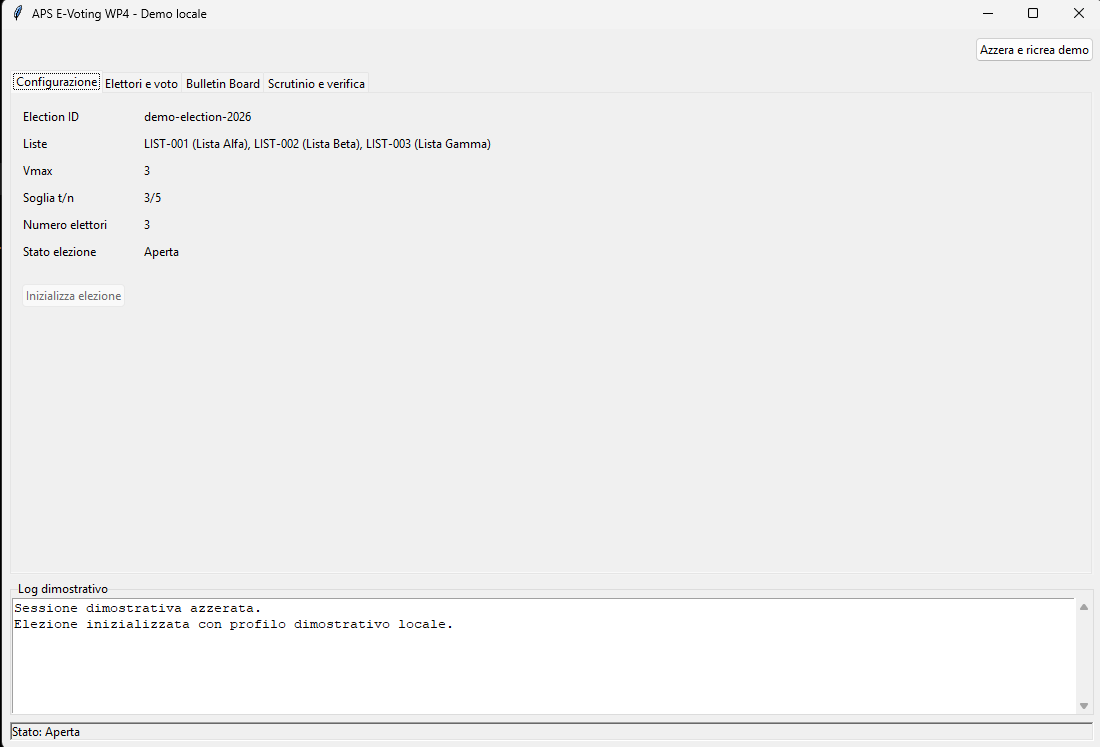
\includegraphics[width=0.92\textwidth]{Figures/gui-configurazione.png}
\caption{Configurazione iniziale del profilo dimostrativo: liste ammesse, limite Vmax, soglia Shamir ed elettori.}
\label{wp4:fig-gui-configurazione}
\end{figure}

\begin{figure}[H]
\centering
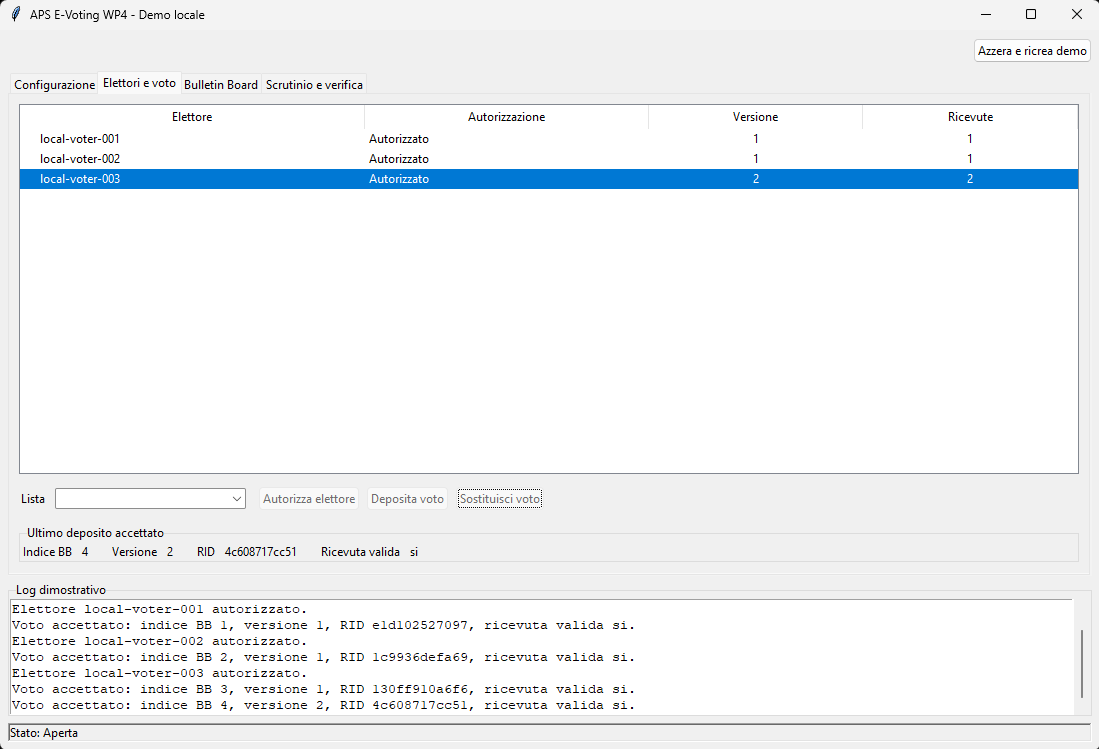
\includegraphics[width=0.92\textwidth]{Figures/gui-elettori-voto.png}
\caption{Stato degli elettori dopo tre depositi e una sostituzione del voto.}
\label{wp4:fig-gui-elettori-voto}
\end{figure}

\begin{figure}[H]
\centering
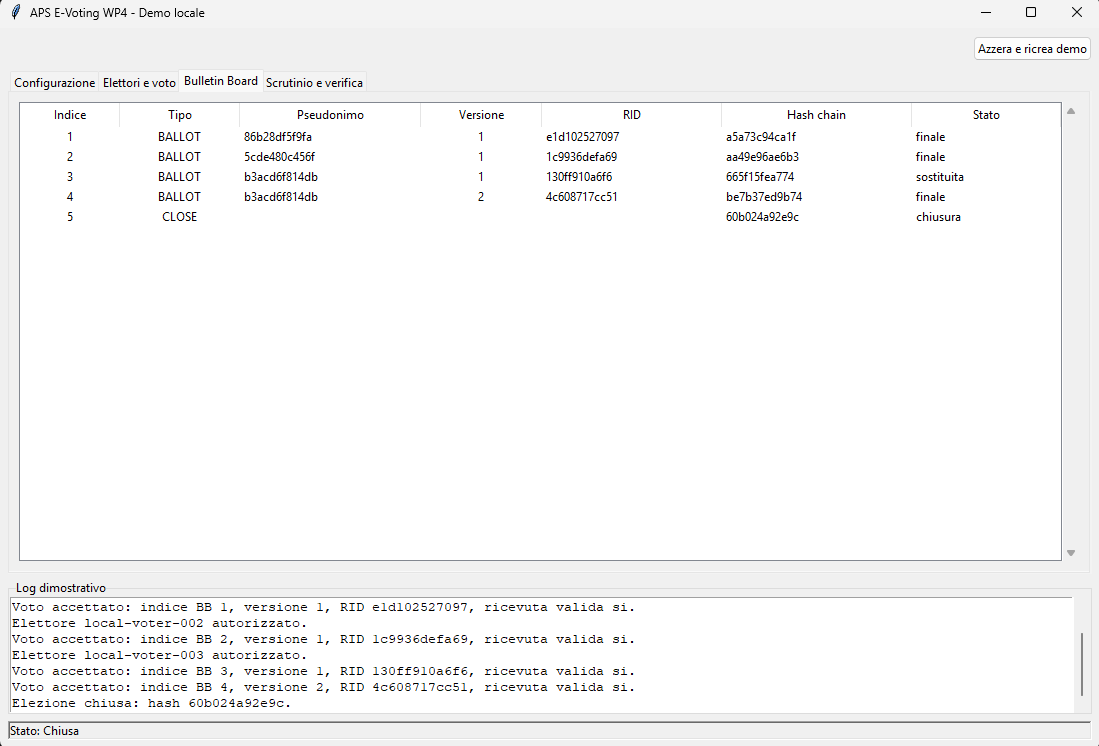
\includegraphics[width=0.92\textwidth]{Figures/gui-bulletin-board.png}
\caption{Bulletin Board dopo la sostituzione e la chiusura: record BALLOT, versione sostituita e record CLOSE.}
\label{wp4:fig-gui-bulletin-board}
\end{figure}

\begin{figure}[H]
\centering
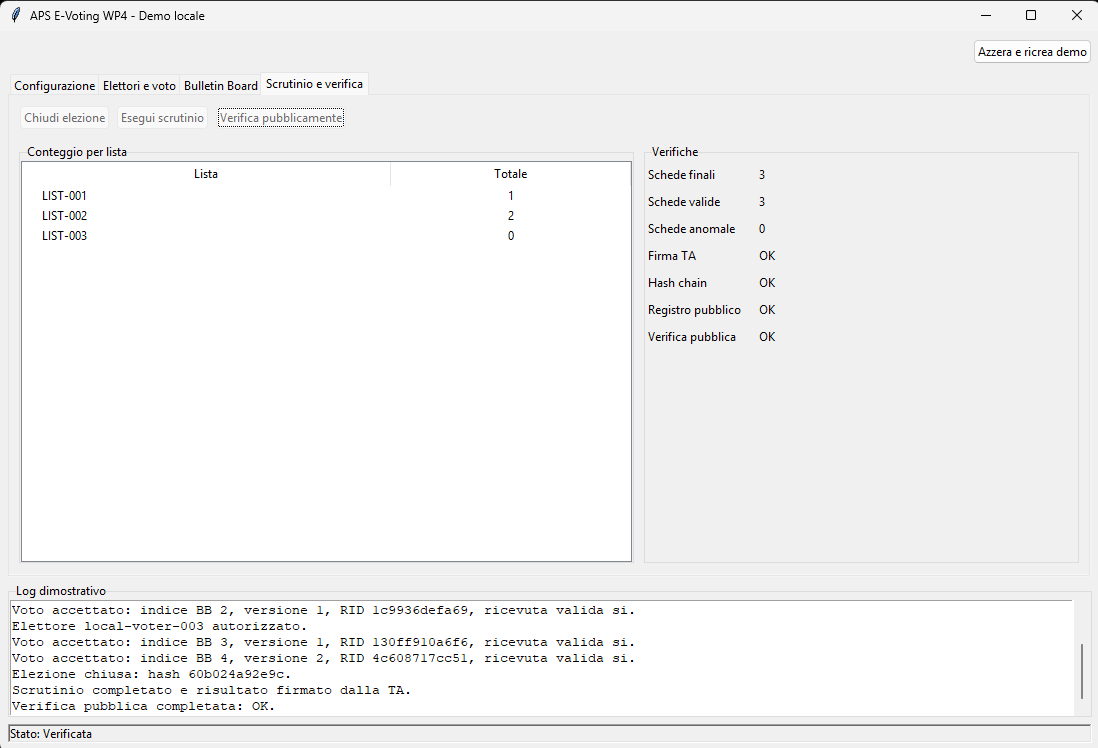
\includegraphics[width=0.92\textwidth]{Figures/gui-scrutinio-verifica.png}
\caption{Risultato dello scrutinio e completamento delle verifiche pubbliche.}
\label{wp4:fig-gui-scrutinio-verifica}
\end{figure}

\subsection{Strategia e risultati dei test}
\label{wp4:test}

La suite finale contiene 282 test superati. La copertura \`e organizzata in quattro gruppi principali.

\begin{itemize}
\item Test unitari: modelli, serializzazione canonica, hash, cifratura RSA-OAEP, firme RSA-PSS, password, Shamir, $\mathit{blob}_{\mathit{TA}}$, stato cifrato dell'elettore e formattazione dei dati pubblici.
\item Test di integrazione: workflow completo, registrazione, autorizzazione, voto, sostituzione, chiusura, scrutinio, verifica individuale, verifica pubblica e flusso GUI locale.
\item Test di sicurezza: alterazione dei parametri pubblici, firma TA errata o prodotta con chiave diversa, autorizzazioni contraffatte, firme modificate, replay, versioni non valide, superamento di $V_{\max}$, voto dopo $\texttt{CLOSE}$, hash chain manomessa, quote Shamir duplicate o malformate, $\mathit{blob}_{\mathit{TA}}$ alterato, MAC non valido, ciphertext malformati e plaintext fuori dominio.
\item Test benchmark: profilo rapido per verificare schema dei risultati, metriche non negative e assenza di dati riservati negli output di misura.
\end{itemize}

Sono inclusi test specifici sulla perdita o corruzione dello stato elettore. Tali casi verificano che la sostituzione non possa essere prodotta senza lo stato locale valido, che la RA rifiuti una seconda autorizzazione e che la scheda gi\`a accettata resti disponibile per lo scrutinio.

\subsection{Benchmark e valutazione delle prestazioni}
\label{wp4:benchmark}

I benchmark sono stati eseguiti con Python 3.14.5 su Windows 11 Home 64 bit, Intel Core i7-12700H e 16 GB di RAM. Il profilo completo usa una fase di warm-up e 5 ripetizioni per le operazioni temporali; i tempi sono riportati in millisecondi. I valori seguenti riprendono le mediane e le dimensioni indicate nel report sperimentale, senza ricalcoli.

\begin{table}[H]
\centering
\resizebox{\textwidth}{!}{%
\begin{tabular}{>{\raggedright\arraybackslash}p{5.1cm}
                >{\raggedright\arraybackslash}p{4.7cm}
                r
                r}
\toprule
\textbf{Operazione} & \textbf{Input / scala} & \textbf{Mediana ms} & \textbf{Dimensione byte} \\
\midrule
Generazione chiave RSA per firma & $2048$ bit & 37.8399 & 0 \\
Generazione chiave RSA per cifratura & $2048$ bit & 46.8595 & 0 \\
Autenticazione e autorizzazione RA & $scrypt\_n=32768$ & 93.3756 & 256 \\
Cifratura RSA-OAEP del voto & plaintext di 8 byte & 0.0263 & 256 \\
Firma RSA-PSS del pacchetto & messaggio di 1114 byte & 0.4765 & 256 \\
Preparazione completa del pacchetto & singolo pacchetto voto & 30.6746 & 1814 \\
Validazione e accettazione BB & singolo pacchetto voto & 1.0974 & 1814 \\
Aggiornamento hash chain & singolo collegamento & 0.0287 & 1966 \\
Verifica ricevuta BB & singola ricevuta & 0.0441 & 568 \\
Suddivisione Shamir & soglia $3$, quote $5$, segreto 32 byte & 0.0083 & 0 \\
Ricostruzione Shamir & soglia $3$, quote fornite $3$ & 0.0073 & 0 \\
Creazione $\mathit{blob}_{\mathit{TA}}$ & chiave privata serializzata di 1704 byte & 0.0786 & 162 \\
Apertura $\mathit{blob}_{\mathit{TA}}$ & soglia $3$, quote fornite $3$ & 0.0607 & 162 \\
Scrutinio & 10 schede finali & 35.2956 & 614 \\
Dimensione pacchetto voto & singolo pacchetto voto & 0.0000 & 1814 \\
Dimensione ricevuta & singola ricevuta & 0.0000 & 568 \\
\bottomrule
\end{tabular}%
}
\caption{Benchmark WP4: sintesi delle operazioni principali.}
\label{wp4:tab-benchmark-operazioni}
\end{table}

Le righe relative alla dimensione del pacchetto e della ricevuta non rappresentano operazioni temporali; per questo motivo il tempo \`e riportato come $0.0000$ ms. Anche la generazione delle chiavi RSA \`e misurata separatamente e non viene sommata alle operazioni ordinarie di voto.

\begin{table}[H]
\centering
\begin{tabular}{r r r r r r}
\toprule
\textbf{Eventi} & \textbf{Rip.} & \textbf{Min ms} & \textbf{Mediana ms} & \textbf{Media ms} & \textbf{Dev. std ms} \\
\midrule
2  & 5 & 0.2966 & 0.3082 & 0.3271 & 0.0531 \\
4  & 5 & 0.5810 & 0.6007 & 0.5985 & 0.0159 \\
11 & 5 & 1.5735 & 1.6055 & 1.7260 & 0.1914 \\
26 & 5 & 3.9386 & 3.9958 & 4.1199 & 0.2329 \\
\bottomrule
\end{tabular}
\caption{Benchmark WP4: verifica pubblica su registri di dimensione crescente.}
\label{wp4:tab-benchmark-verifica-pubblica}
\end{table}

La verifica pubblica cresce in modo coerente con il numero di eventi esaminati, poich\'e il verificatore ricalcola record, firme, $\mathit{RID}_i$, hash chain, versioni, selezione finale e coerenza numerica. I risultati devono tuttavia essere letti come misure del prototipo locale e non come stima di un sistema distribuito reale.

\subsection{Limiti del prototipo}
\label{wp4:limiti}

Il prototipo conserva limiti espliciti. La verifica pubblica della corretta decifratura resta parziale: registro, firme, versioni, $V_{\max}$, selezione finale, legame con $h_{\mathit{close}}$, firma TA e coerenza numerica sono controllabili, ma non sono presenti prove pubbliche della corretta decifratura di ogni scheda.

Non \`e implementata una vera threshold decryption. Shamir protegge $K_{\mathit{wrap}}$, ma durante lo scrutinio la chiave privata di decifratura della TA viene ricostruita temporaneamente nell'ambiente della TA. La GUI ha finalit\`a dimostrativa e non sostituisce un'interfaccia di produzione. La persistenza \`e limitata allo scenario locale e non include un database distribuito o politiche operative complete. I benchmark, infine, sono stati raccolti su una singola macchina e non rappresentano latenza di rete, concorrenza reale, isolamento tra server o carichi di un'infrastruttura distribuita.

\subsection{Considerazioni conclusive}
\label{wp4:conclusioni}

Il WP4 mostra che il protocollo descritto nei WP precedenti pu\`o essere implementato in un prototipo locale coerente con le propriet\`a progettuali principali. La separazione logica degli attori, l'uso di serializzazione canonica, firme, cifratura probabilistica, registro append-only, Shamir su $K_{\mathit{wrap}}$, persistenza cifrata dello stato elettore e verifiche pubbliche consentono di esercitare l'intero workflow in modo riproducibile.

La suite di test conferma il comportamento atteso nei casi ordinari e in numerosi casi negativi. I benchmark indicano costi contenuti per le operazioni locali misurate, con particolare attenzione alla separazione tra primitive crittografiche, operazioni applicative e verifica pubblica. Le limitazioni dichiarate rimangono sostanziali e impediscono di interpretare il prototipo come sistema elettorale reale; esso costituisce invece una validazione didattica e sperimentale del disegno protocollare.


\end{document}
